\documentclass[lettersize,journal]{IEEEtran}
\def\MakeUppercaseUnsupportedInPdfStrings{\scshape}
    
\usepackage{amsmath,amsfonts}
\usepackage{algorithmic}
\usepackage{algorithm}
\usepackage{array}
\usepackage[caption=false,font=normalsize,labelfont=sf,textfont=sf]{subfig}
\usepackage{textcomp}
\usepackage{stfloats}
\usepackage{url}
\usepackage{hyperref}
\usepackage{verbatim}
\usepackage{graphicx}
\usepackage[backend=bibtex]{biblatex}
\usepackage[utf8]{inputenc}
\usepackage{pgfplots}
\usepackage{tikz}
\usepackage{siunitx}

\addbibresource{refs.bib}
\graphicspath{{images/block_design/CP/}}

\begin{document}

\title{Simulation and Design of a SpaceFibre 6.25 GHz PLL}

\author{Alessandro Porta, \texttt{a.porta2@studenti.unipi.it}\\
Leonardo Bove, \texttt{l.bove3@studenti.unipi.it}\\
Department of Information Engineering (DII), University of Pisa, Pisa}


\maketitle

\begin{abstract}
This paper presents the design and analysis of a Type-II charge pump Phase-Locked Loop (PLL) operating at \(6.25 \, \text{GHz}\), compatible with the SpaceFibre standard. A system-level analysis was conducted to dimension the components, ensuring stability, phase margin, and bandwidth. The key building blocks, including the phase-frequency detector, charge pump (implemented in SG25H4 technology), and loop filter, were designed, tested, and validated.

The proposed PLL demonstrates both phase and frequency locking with satisfactory dynamic behavior, as confirmed through simulations against an ideal implementation. The impact of VCO phase noise was analyzed, revealing the expected high-pass characteristic of the closed-loop phase noise response. A comparison with a Type-I PLL highlights the superior capability of the Type-II PLL to achieve phase and frequency locking.

This work establishes the robustness of the Type-II charge pump PLL in meeting the stringent requirements of high-performance standards such as SpaceFibre.
\end{abstract}

\section{Introduction}
\IEEEPARstart{I}{nter-satellite} communication is increasingly critical for modern space applications, demanding high data rates, low latency, and robust signal integrity. The SpaceFibre standard addresses these requirements by defining high-speed communication protocols suitable for the harsh conditions of space. At the core of this implementation lies the Phase-Locked Loop (PLL), essential for clock recovery and data synchronization, operating at frequencies up to \(6.25 \, \text{GHz}\). 

This work focuses on designing a PLL in the SG25H4 technology that meets the stringent requirements of the SpaceFibre standard. Initially, behavioral models for the Phase-Frequency Detector (PFD) and Charge Pump (CP), along with an idealized Voltage-Controlled Oscillator (VCO), are used to evaluate system-level performance. This includes detailed analysis of transient behavior, dynamic response to disturbances, and stability characteristics.

Subsequently, these behavioral models are replaced with physically implemented designs for the PFD and CP. The PFD is realized using D flip-flops, while the CP employs an actual current source circuit. This transition highlights the impact of real-world non-idealities on PLL performance, offering insights into design challenges and optimization strategies.

The combination of system-level analysis and physical implementation provides a comprehensive framework for developing high-frequency PLLs tailored to SpaceFibre, paving the way for future advancements in satellite communication systems.

This work is organized as follows: Section~\ref{sec:system_architecture_and_analysis} provides an overview of the main components of a charge pump PLL, including the system-level design and analysis. Section~\ref{sec:block_design} focuses on the design of individual component blocks and the tests conducted for each one. Section~\ref{sec:ADS_simulations} presents the ADS simulations of the complete PLL, starting with behavioral models and then incorporating the designed blocks. Section~\ref{sec:comparison} shows a comparison between this work type-II charge pump PLL and a Type-I phase detector PLL. Section~\ref{sec:future_improvements} discusses possible directions for future research. Finally, Section~\ref{sec:conslusions} concludes and summarizes the results obtained.

It is important to note that this work focuses solely on evaluating and designing potential building blocks of a PLL for the SpaceFibre standard, without considerations for layout implementation or post-layout analysis.

This work is based on research conducted at the University of Pisa, focusing on the analysis and design of integrated blocks for a 6.25 GHz SpaceFibre Phase-Locked Loop (PLL) implemented using 65 nm CMOS technology \cite{original}. The study builds upon the foundational work carried out at the university to explore system-level and circuit-level design considerations for high-frequency applications, with particular attention to meeting the stringent requirements of the SpaceFibre standard. This includes achieving low phase noise, robust operation in radiation-prone environments, and compliance with performance metrics suitable for space-grade systems.

\subsection{The Standard SpaceFibre}

The Standard SpaceFibre was released by the European Space Agency in 2019 to define high-speed communication protocols suitable for space environments. It supports data transmission for high-bandwidth sensors up to 6.25 Gbps, with the PLL being a key block for its implementation. The PLL must be hardened against Single Event Effects (SEE) and Total Ionizing Dose (TID) radiation effects, operate within a temperature range of -55°C to 125°C, and sustain frequencies up to 6.25 GHz.

This work, however, focuses on designing a Phase-Locked Loop (PLL) using 250 nm SiGe technology at 6.25 GHz, without specific consideration for radiation-hardening, which could be addressed in future work. For example, radiation-hardening often comes at the cost of increased power and area consumption due to the implementation of redundancy techniques. Currently, Triple Modular Redundancy (TMR) is one of the most effective techniques for digital blocks, such as the Phase-Frequency Detector (PFD). TMR involves triplicating a cell and adding a voter circuit to determine the majority output.

For the Charge Pump (CP), voltage-switching Charge Pumps (V-CP) have been shown to effectively mitigate SEE, but they significantly degrade noise performance compared to standard CP designs. Addressing such trade-offs is a key challenge for future radiation-hardened PLL implementations.

\section{System Architecture and Analysis}
\label{sec:system_architecture_and_analysis}
PLLs represent the feedback control systems that find very broad applications in communication systems, clock generation, and synchronization applications. In general, a PLL aims to provide the phase and frequency of an output signal identical to a reference signal in a very stable and accurate way at high speeds. This is attained in PLL through the constant control of a VCO frequency with the phase difference between a reference and feedback signal as shown in Fig.~\ref{fig:simple_pll}.

\begin{figure}[!h]
    \centering
    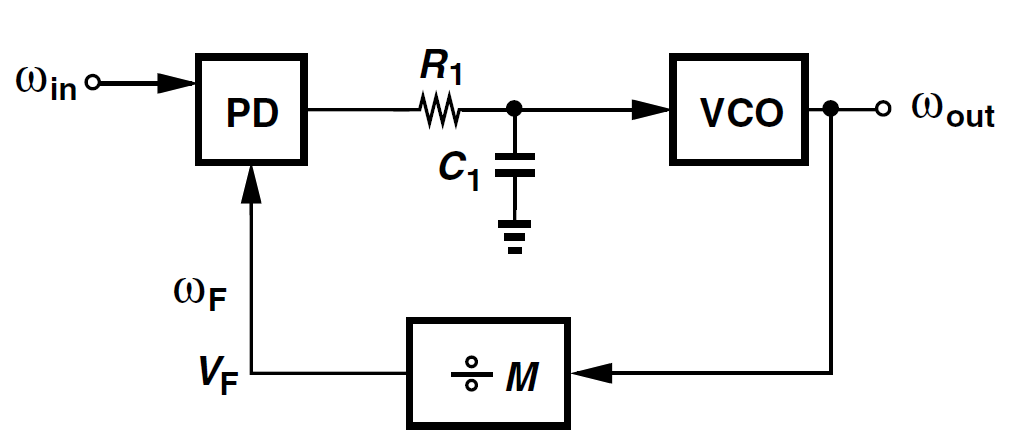
\includegraphics[width=0.75\linewidth]{images/intro_system_level/simple_pll.png}
    \caption{Simple PLL implementation.}
    \label{fig:simple_pll}
\end{figure}

However, in this work, we focus on a more sophisticated PLL design, specifically a charge pump PLL (CP-PLL). This architecture offers superior performance compared to simpler PLL designs, particularly in terms of noise reduction and stability, making it better suited for high-frequency applications such as the SpaceFibre standard.

\begin{figure}[!h]
    \centering
    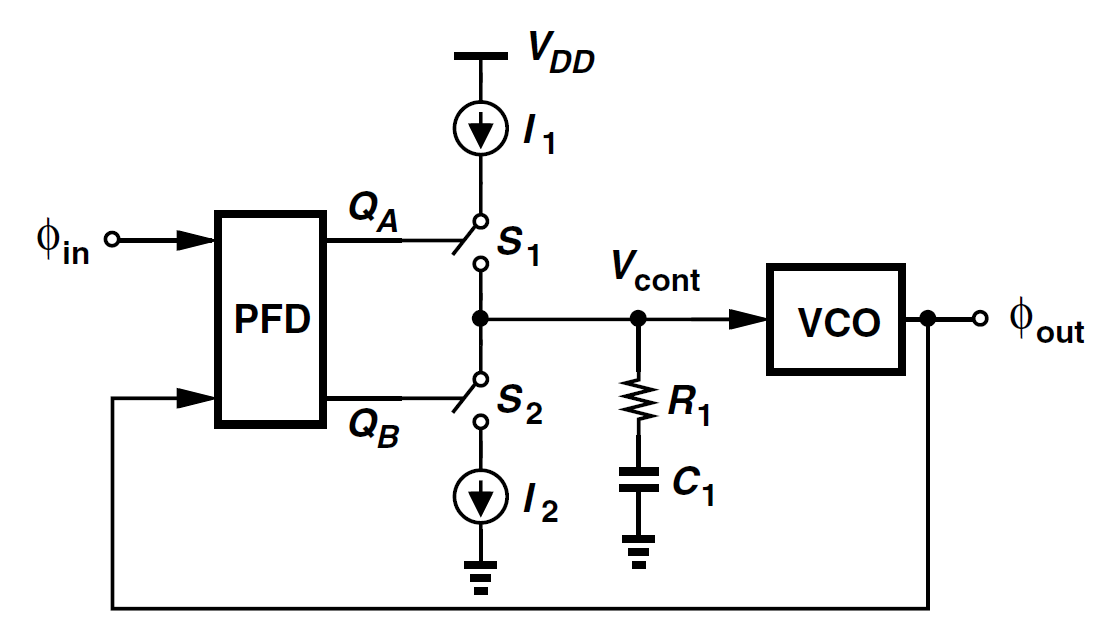
\includegraphics[width=0.75\linewidth]{images/intro_system_level/pll_cp.png}
    \caption{CP-PLL implementation.}
    \label{fig:pll_cp}
\end{figure}

The fundamental blocks of a charge pump PLL (shown in Fig.~\ref{fig:pll_cp}) are as follows:

\begin{itemize}
    \item \textbf{Phase-Frequency Detector}: The phase detector compares the phase of the reference signal with the feedback signal from the PLL output. It generates an output proportional to the phase difference, which serves as an error signal for the control loop. A PFD extends this functionality by also detecting frequency differences, enabling faster acquisition of lock.
    \item \textbf{Charge Pump}: The charge pump converts the phase error signal from the PFD into a current signal. Depending on the phase difference, it sources or sinks current to drive the loop filter. It acts as a very critical component in shaping the loop's dynamic response and maintaining stable operation.
    \item \textbf{Loop Filter}: This smooths the charge pump output, generating a VCO control voltage. The loop filter usually consists of low-pass filter components, in order to lower high-frequency noise, where the bandwidth and stability of the PLL along with transient response is determined. 
    \item \textbf{Voltage-Controlled Oscillator (VCO)}: The VCO generates the output signal whose frequency is controlled by the input voltage from the loop filter. The most important parameters in the VCO of the PLL are the VCO's tuning range and linearity.
    \item \textbf{Frequency Divider}: In most of the PLL architectures, the feedback path contains a frequency divider that divides the output frequency of the VCO. The reference frequency could then actually be a sub-multiple of the VCO output frequency at which the PLL can lock, allowing greater flexibility in the synthesis of output frequencies.
\end{itemize}

The PLL works in such a way that it varies the frequency of the VCO until the phase difference between the reference and feedback signals is at a minimum. At the point of steady state, the loop acquires a phase lock where the output frequency equals the reference frequency, or is a multiple of it if there is a divider. The interaction of these components will define the acquisition time, stability, and jitter performance of the PLL, which are important metrics in high-speed communication systems.

\subsection{System Level Design and Analysis}
\label{sec:system_level_analysis}

\begin{figure}[!h]
    \centering
    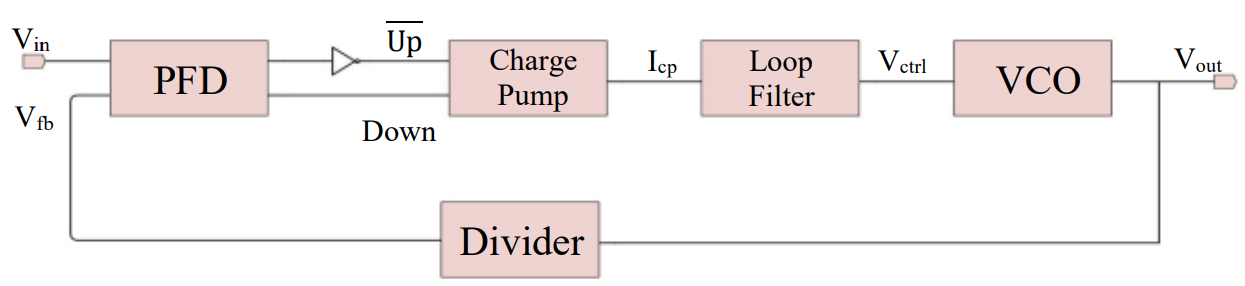
\includegraphics[width=1\linewidth]{images/intro_system_level/pll_block_diagram.png}
    \caption{PLL system block diagram.}
    \label{fig:pll_block_diagram}
\end{figure}

\begin{figure*}[!ht]
    \centering
    \subfloat[]{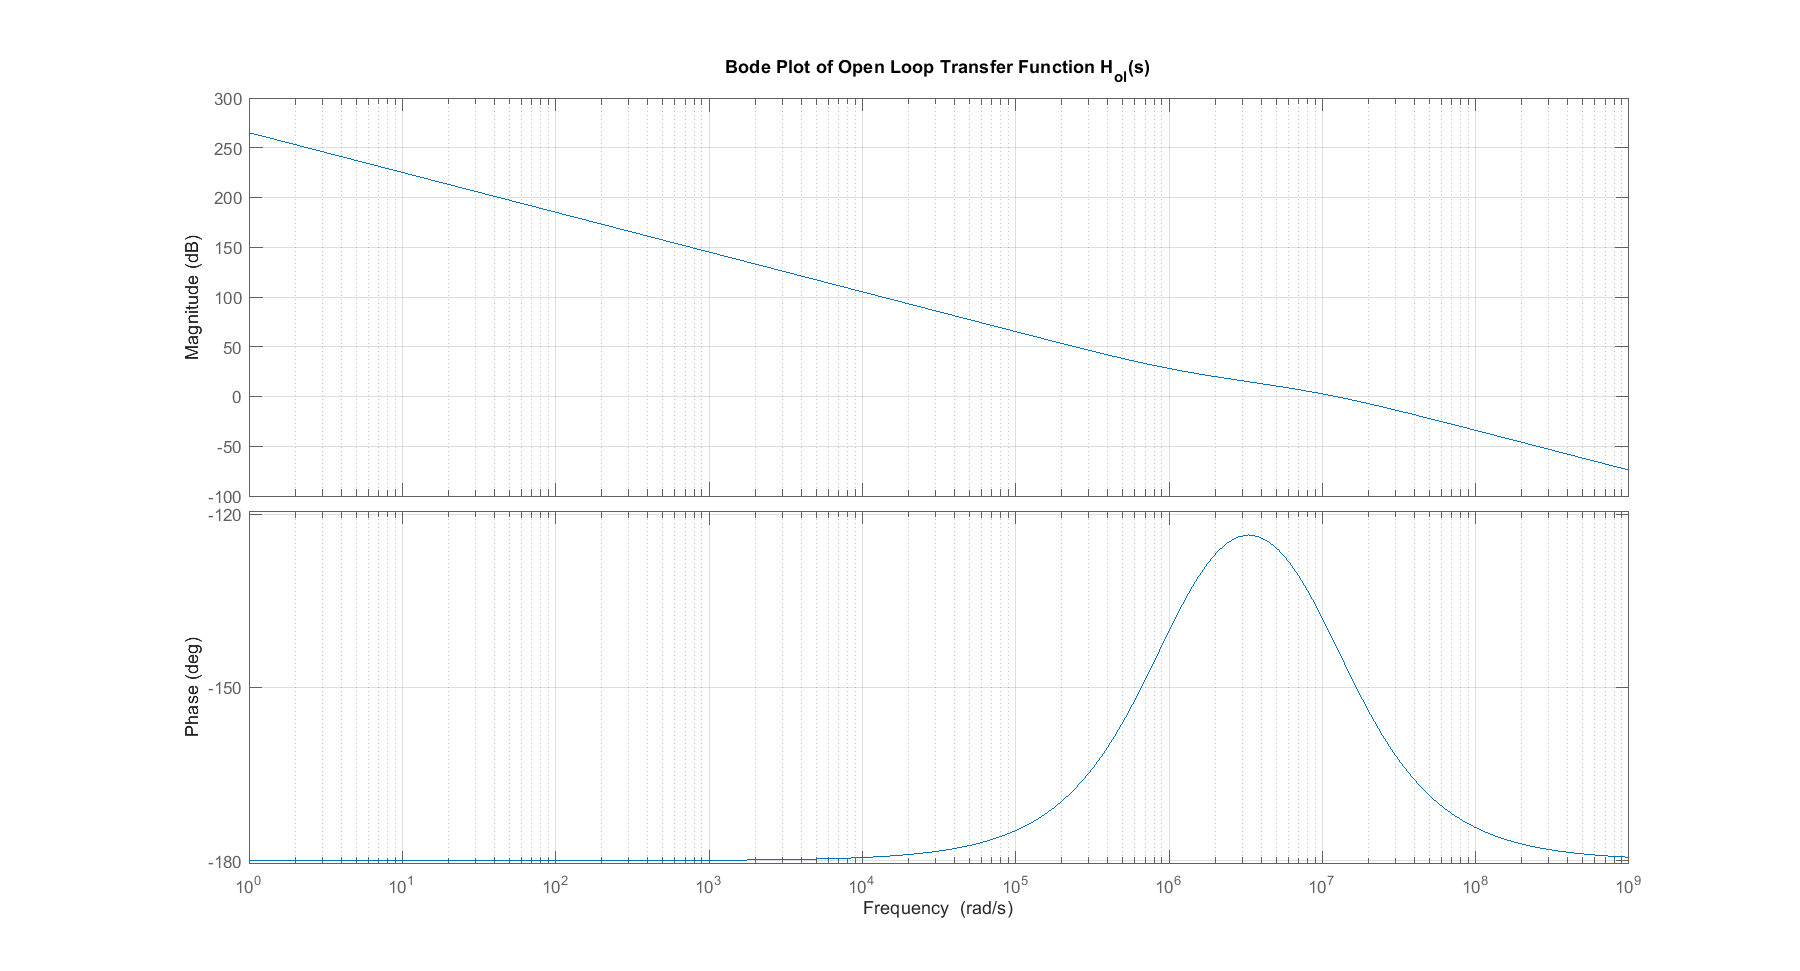
\includegraphics[width=0.5\linewidth]{images/bode_plots/OL_bode.png}%
    \label{fig:OL_bode}}
    \hfil
    \subfloat[]{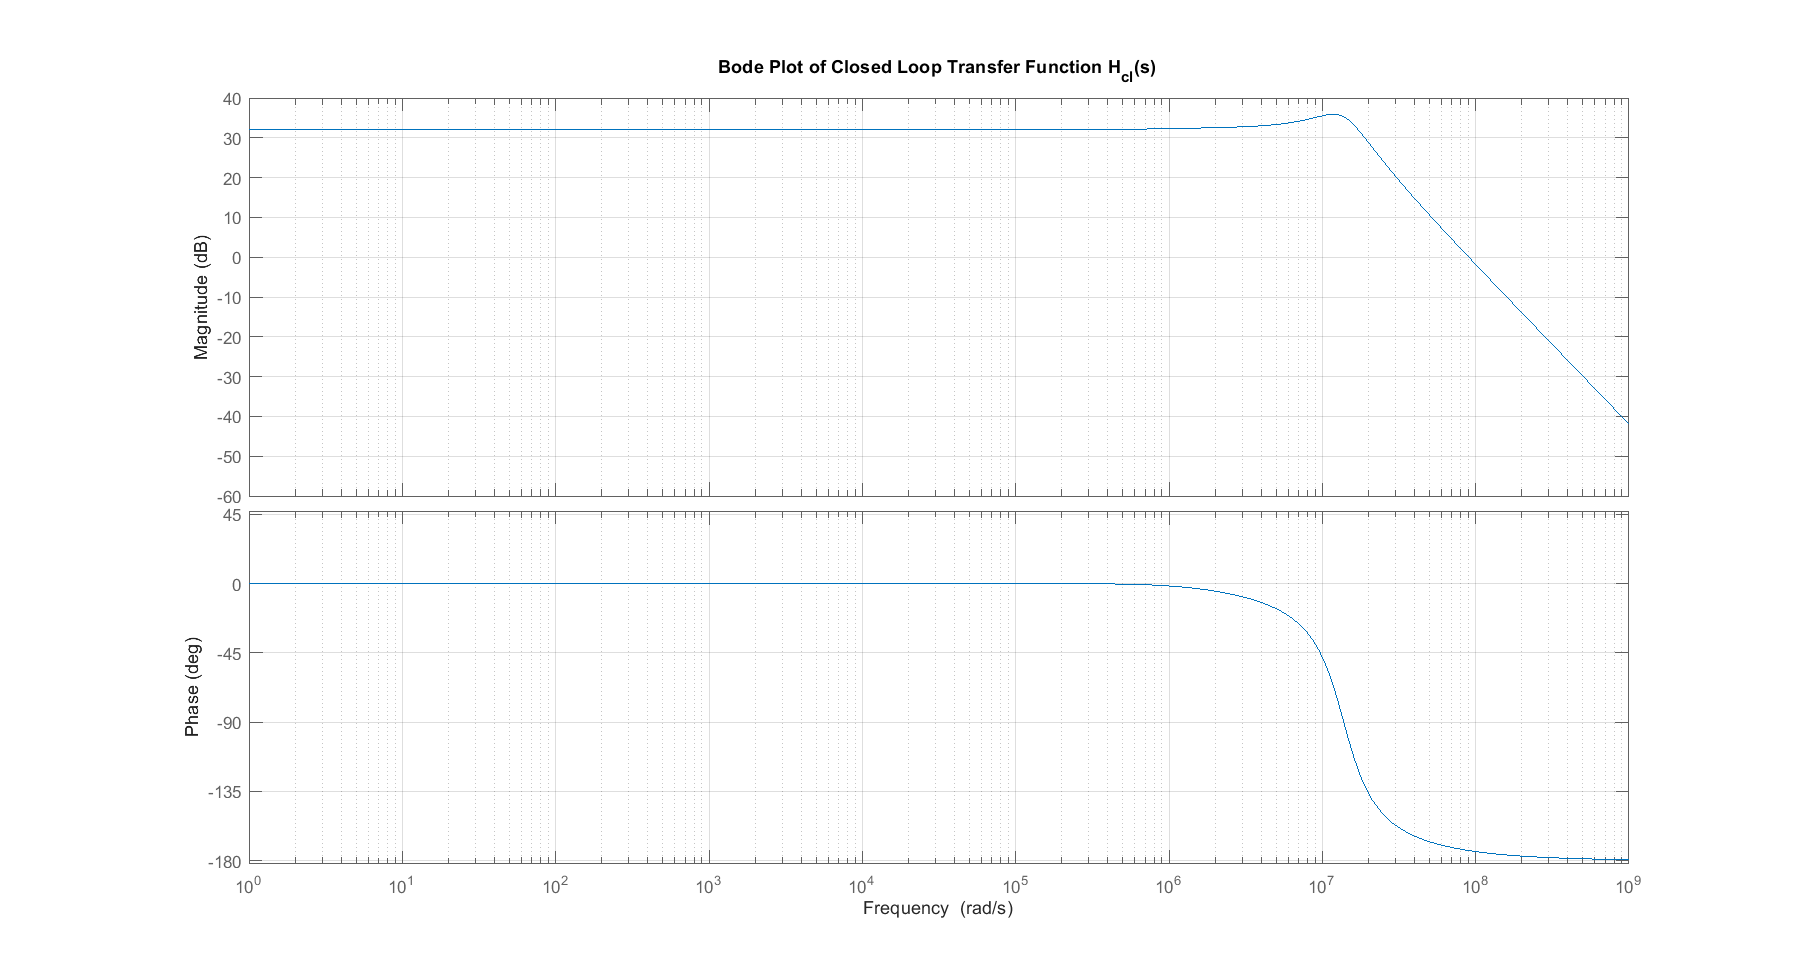
\includegraphics[width=0.5\linewidth]{images/bode_plots/CL_bode.png}%
    \label{fig:CL_bode}}
    \hfil
    \caption{Bode plots, (a) Open loop, (b) Closed loop.}
    \label{fig:bode_plots}
\end{figure*}

Figure~\ref{fig:pll_block_diagram} shows a classical charge pump Phase-Locked Loop (CP-PLL) block schematic. All blocks, except for the Voltage-Controlled Oscillator (VCO), operate at a lower frequency due to the frequency divider. In this work, we have the following parameters:

\begin{itemize}
    \item \( N = 40 \) as the frequency divider,
    \item \( f_{\text{vco}} = 6.25 \, \text{GHz} \), the output frequency as set in the standard SpaceFibre,
    \item \( f_{\text{ref}} = \frac{f_{\text{vco}}}{N} = 156.25 \, \text{MHz} \), the reference frequency at which the PLL operates,
    \item \( f_0 = 5.95 \, \text{GHz} \), the frequency at which the VCO works.
\end{itemize}

According to the SpaceFibre standard, the PLL must also generate frequencies of \( 3.125 \, \text{GHz} \) and \( 1.5625 \, \text{GHz} \). These frequencies are achieved using an integer frequency divider with division ratios as follows:

\begin{itemize}
    \item \( \frac{1}{2} \) for \( 3.125 \, \text{GHz} \),
    \item \( \frac{1}{4} \) for \( 1.5625 \, \text{GHz} \),
    \item \( \frac{1}{40} \) for the main frequency divider.
\end{itemize}

However, in this work, the first two dividers are not included, as their implementation is outside the scope of this study.

\subsubsection{Phase-domain model}
Given this, it is necessary to develop a phase-domain model to analyze the bandwidth and stability of the PLL designed in this work. At this stage, all the blocks are linearized for small signals, and we refer again to Fig.~\ref{fig:pll_block_diagram}. The following describes the behavior of each block:

\begin{itemize}
    \item \textbf{Phase Frequency Detector/Charge Pump (PFD/CP):} The PFD/CP has a constant gain of \( \frac{I_{\text{CP}}}{2\pi} \). The output current of the charge pump is given by 
    \[ 
    I_e = \frac{I_{\text{CP}}}{2\pi} \left( \theta_{\text{ref}} - \theta_{\text{fb}} \right)
    \] 
    where \(I_e\) is the error current, \( \theta_{\text{ref}} \) and \( \theta_{\text{fb}} \) represent the phases of the reference and feedback signals, respectively. Here, \( I_{\text{CP}} = 400~\mu\mathrm{A} \), as discussed in Section~\ref{sec:charge_pump}.
    
    \item \textbf{Frequency Divider:} The frequency divider is modeled with a constant gain of \( \frac{1}{N} \), where \( N = 40 \).
    
    \item \textbf{Loop Filter:} The loop filter is represented as \( Z(s) \), which provides the voltage output of the filter. Its input is the charge pump current, so the voltage at the control input of the VCO is given by 
    \[ 
    V_{\text{ctrl}} = I_e \cdot Z(s) 
    \] 
    The transfer function of the loop filter is given by:
    \[
    Z(s) = \frac{\frac{1}{s(C_1 + C_2)} \left(1 + sRC_1\right)}{1 + sR\frac{C_1C_2}{C_1 + C_2}}
    \]
    The values chosen for the loop filter components will be discussed in Section~\ref{sec:loop_filter}.
    
    \item \textbf{Voltage-Controlled Oscillator (VCO):} The VCO is modeled as an integrator with a gain of \( K_{\text{VCO}} = 2~\mathrm{GHz/V} \), as discussed in Section~\ref{sec:vco}. The frequency output is given by 
    \[ 
    \theta_{\text{vco}}(s) = \frac{K_{\text{VCO}}}{s} \cdot V_{\text{ctrl}} 
    \]
    where \(\theta_{\text{vco}}(s) = N \cdot \theta_{\text{fb}}(s)\) thanks to the frequency divider.
\end{itemize}

Given these linearized models, the open-loop transfer function is:

\begin{equation}
    H_{\text{OL}}(s) =\frac{I_{\text{CP}}}{2\pi} Z(s) \frac{K_{\text{VCO}}}{s} \frac{1}{N}
\end{equation}

The closed-loop transfer function is:

\begin{equation}
    H_{\text{CL}}(s) = \frac{\theta_{\text{vco}}(s)}{\theta_{\text{ref}}(s)} =  \frac{\frac{I_{\text{CP}}}{2\pi} Z(s) \frac{K_{\text{VCO}}}{s}}{1 + \frac{I_{\text{CP}}}{2\pi} Z(s) \frac{K_{\text{VCO}}}{s} \frac{1}{N}}
\end{equation}

These transfer functions provide insight into the system's stability and bandwidth, enabling optimization of the PLL's design parameters.

The evaluations of these transfer functions were carried out using MATLAB to plot the Bode functions and obtain the open-loop phase margin and the closed-loop bandwidth.

As shown in Fig.~\ref{fig:bode_plots}, this model achieves a bandwidth of 5.30~MHz and a phase margin of \( 32^\circ \). It is important to note that a trade-off has been made to balance good dynamic performance, a stable steady-state value, and acceptable phase noise. The latter will be discussed in Section~\ref{sec:phase_noise}.


\section{Blocks Design} 
\label{sec:block_design}

In this section, the implementation and testing of each individual block of the charge pump PLL are described. Each block is designed and tested separately using ADS to ensure proper functionality before integration into the complete PLL system. The tests focus on validating the behavior of each block under the expected operating conditions.

\subsection{Loop Filter}
\label{sec:loop_filter}
\begin{figure}[!h]
    \centering
    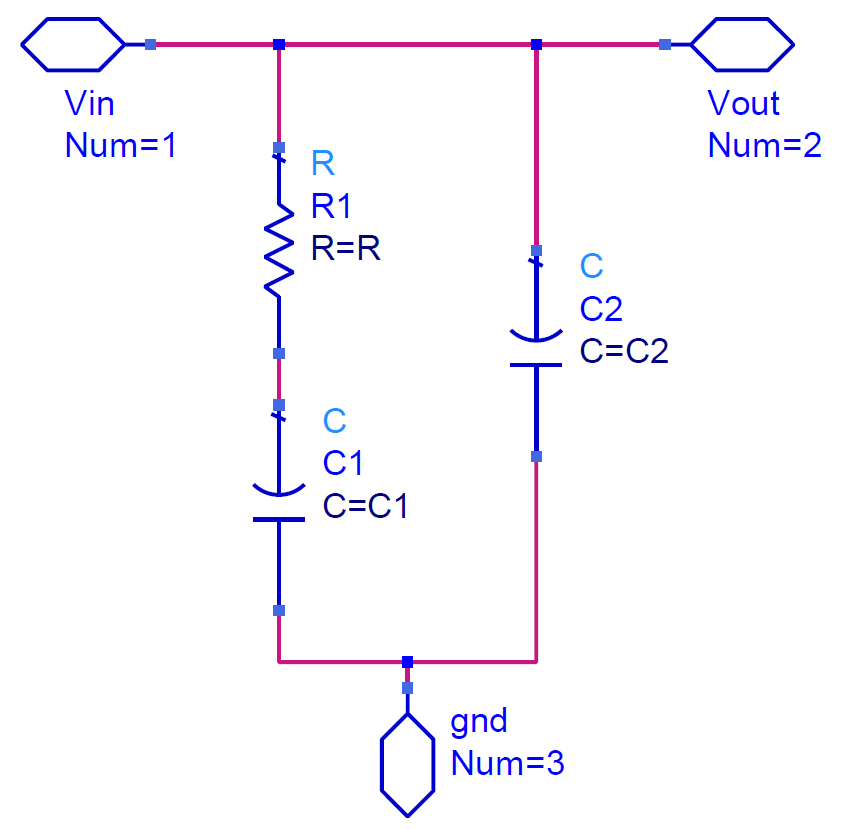
\includegraphics[width=0.5\linewidth]{images/block_design/LOOP_FILTER/loop_filter.png}
    \caption{Second order loop filter implementation.}
    \label{fig:loop_filter}
\end{figure}

The loop filter, shown in Fig.~\ref{fig:loop_filter}, is a second-order low-pass filter selected for this work. It consists of a capacitor \( C_1 \), a resistor \( R \) to stabilize the loop, and a capacitor \( C_2 \). According to~\cite{razavi2011rf}, the purpose of \( C_2 \) is to reduce spurious tones at multiples of the reference frequency. Its value is chosen to be no more than \( C_1/5 \) to achieve the desired performance.

Based on the discussions in Section~\ref{sec:system_level_analysis}, and through fine-tuning performed in MATLAB to optimize feedback performance, the selected component values are: \( R = 1~\mathrm{k\Omega} \), \( C_1 = 1000~\mathrm{pF} \), and \( C_2 = 100~\mathrm{pF} \).

It is important to note that considerations on the integrability of these capacitors must be addressed, as these values may not be directly integrable using the chosen G25H4 technology.

\subsection{Phase-Frequency Detector}

\subsubsection{Design}
The first block to be analyzed is the phase-frequency detector (PFD). Unlike a simple phase detector, the PFD can also detect frequency differences, allowing the system to lock not only to the phase but also to the frequency. 

The PFD circuit produces two primary outputs, \( Q_a \) and \( Q_b \), and operates based on the following principles:
\begin{enumerate}
    \item A rising edge on \( A \) yields a rising edge on \( Q_a \) (if \( Q_a \) is low).
    \item A rising edge on \( B \) resets \( Q_a \) (if \( Q_a \) is high).
\end{enumerate}
The circuit is symmetric with respect to \( A \) and \( B \) (and \( Q_a \) and \( Q_b \)). 

If \( \omega_A > \omega_B \), \( Q_a \) generates pulses while \( Q_b \) remains at zero. Conversely, if \( \omega_B > \omega_A \), positive pulses appear at \( Q_b \) while \( Q_a = 0 \). On the other hand, if \( \omega_A = \omega_B \), the circuit generates pulses at either \( Q_a \) or \( Q_b \) with a width equal to the phase difference between \( A \) and \( B \). Thus, the average value of \( Q_a - Q_b \) represents the frequency or phase difference.

To better understand the operation of the PFD, Fig.~\ref{fig:PFD_FSM} shows the finite state machine (FSM) summarizing its operation. If the PFD is in state 0, a transition on \( A \) moves it to state I, where \( Q_a = 1 \), \( Q_b = 0 \). The circuit remains in this state until a transition occurs on \( B \), upon which the PFD returns to state 0. The switching sequence between states 0 and II is similar. 

\begin{figure}[!h]
    \centering
    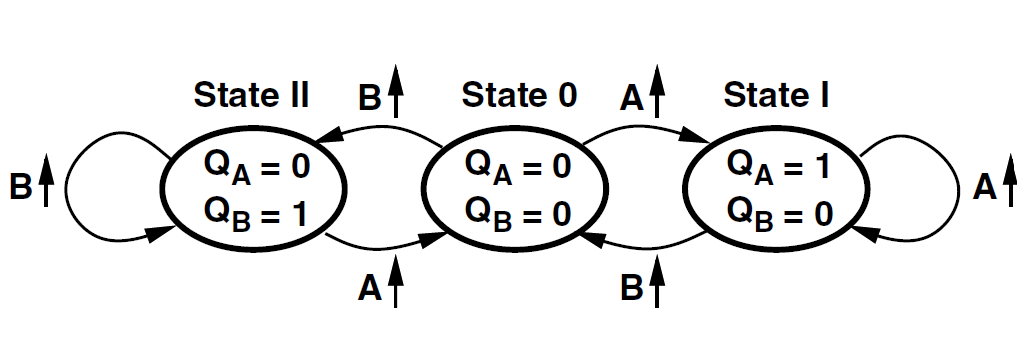
\includegraphics[width=0.75\linewidth]{images/block_design/PFD/PFD_FSM.png}
    \caption{FSM showing desired operation of PFD.}
    \label{fig:PFD_FSM}
\end{figure}

Figure~\ref{fig:PFD} illustrates the logical implementation of the described FSM. 

\begin{figure}[!h]
    \centering
    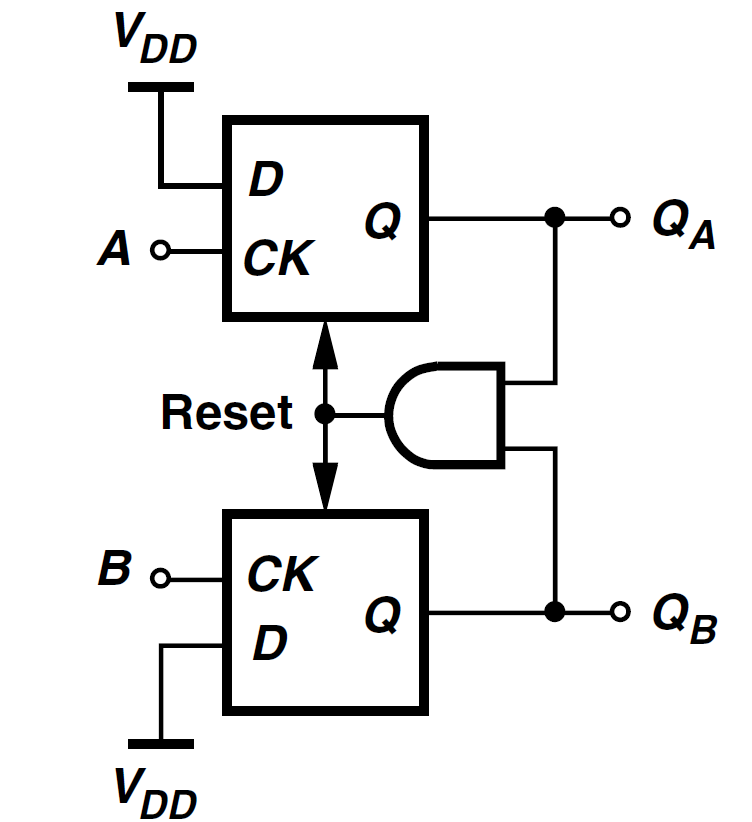
\includegraphics[width=0.4\linewidth]{images/block_design/PFD/PFD.png}
    \caption{PFD implementation.}
    \label{fig:PFD}
\end{figure}

The two inputs to the PFD are:
\begin{itemize}
    \item The reference frequency (\( A \)), a pulse signal with a period \( T = \frac{1}{f_{\text{ref}}} \), where \( f_{\text{ref}} = 156.25~\mathrm{MHz} \).
    \item The feedback signal (\( B \)), a pulse signal derived from the VCO output divided by 40.
\end{itemize}

The circuit consists of two edge-triggered, resettable D flip-flops with their \( D \) inputs tied to logical ONE. Signals \( A \) and \( B \) act as clock inputs for \( \text{DFF}_A \) and \( \text{DFF}_B \), respectively. An AND gate resets the flip-flops when \( Q_a = Q_b = 1 \).

A transition on \( A \) forces \( Q_a \) to be equal to the \( D \) input, i.e., logical ONE. Subsequent transitions on \( A \) have no effect. When \( B \) goes high, \( Q_b \) is also set high, activating the reset of the flip-flops. Thus, \( Q_a \) and \( Q_b \) are simultaneously high for a duration determined by the total delay through the AND gate and the reset path of the flip-flops.

To ensure compatibility with the subsequent block, the charge pump, complementary signals \( Q_{a\_n} \) and \( Q_{b\_n} \) are also generated alongside \( Q_a \) and \( Q_b \).

\begin{figure}[!h]
    \centering
    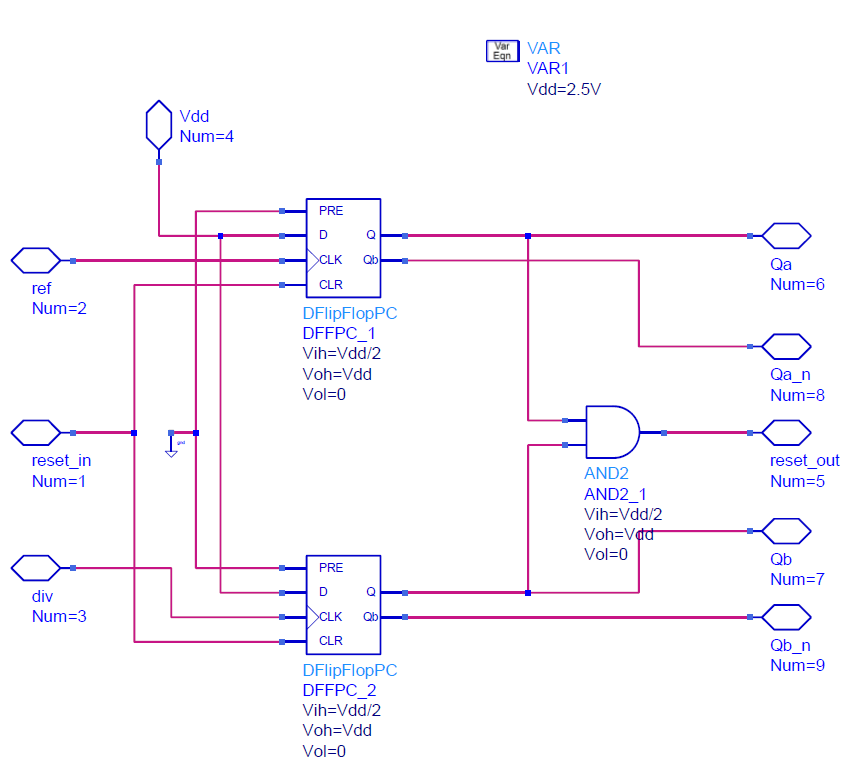
\includegraphics[width=1\linewidth]{images/block_design/PFD/PFD_ADS.png}
    \caption{PFD implementation.}
    \label{fig:PFD_ADS}
\end{figure}

Figure~\ref{fig:PFD_ADS} illustrates the ADS implementation of the PFD. The input ports are:
\begin{itemize}
    \item \textbf{ref}: This represents the reference signal (\( A \) in the previous description).
    \item \textbf{div}: This corresponds to the feedback signal (\( B \) previously named).
\end{itemize}

Additionally, the \textbf{reset} is included as an input in this implementation. This design choice provides flexibility for future enhancements, such as the inclusion of a triple modular redundancy (TMR) system as described later in section~\ref{sec:future_improvements}. In the present work, the \texttt{reset\_in} is simply connected to \texttt{reset\_out} at a higher hierarchical level.

Moreover, for the D flip-flops used in this design, considering a power supply of \( V_{DD} = 2.5\,\mathrm{V} \), the input high voltage (\( V_{IH} \)) is set to \( V_{DD}/2 \), corresponding to \( 1.25\,\mathrm{V} \). The output high voltage (\( V_{OH} \)) is set to \( V_{DD} = 2.5\,\mathrm{V} \), while the output low voltage (\( V_{OL} \)) is set to \( 0\,\mathrm{V} \). These same considerations are also applied to the AND logic block, ensuring consistent voltage levels across the components.

\subsubsection{Test}

\begin{figure*}[!ht]
    \centering
    \subfloat[]{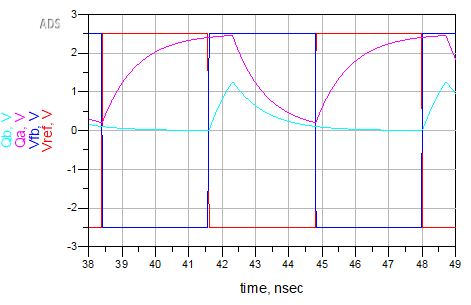
\includegraphics[width=0.5\linewidth]{images/block_design/PFD/PFD_test_50.png}%
    \label{fig:pfd_output_50}}
    \hfil
    \subfloat[]{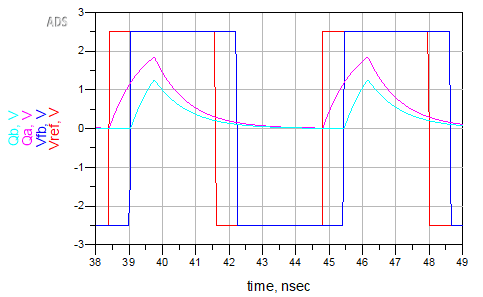
\includegraphics[width=0.5\linewidth]{images/block_design/PFD/PFD_test_10.png}%
    \label{fig:pfd_output_10}}
    \hfil
    \caption{PFD output voltages: (a) and (b) show the time evolution of \(Q_a\) and \(Q_b\) outputs for a positive phase delay (\texttt{Vref} is early compared to \texttt{Vfb}) of $\frac{0.5}{f_{ref}}$ and $\frac{0.1}{f_{ref}}$ respectively.} 
    \label{fig:pfd_test_waveforms}
\end{figure*}

The phase-frequency detector cell was tested in ADS. The inputs for the PFD were connected to two ideal square waves at a frequency of $f_{ref}=\SI{156.25}{\mega\hertz}$ and with a slight phase delay between the two. The testbench used is shown in Fig. \ref{fig:pfd_test}.

\begin{figure}[!ht]
    \centering
    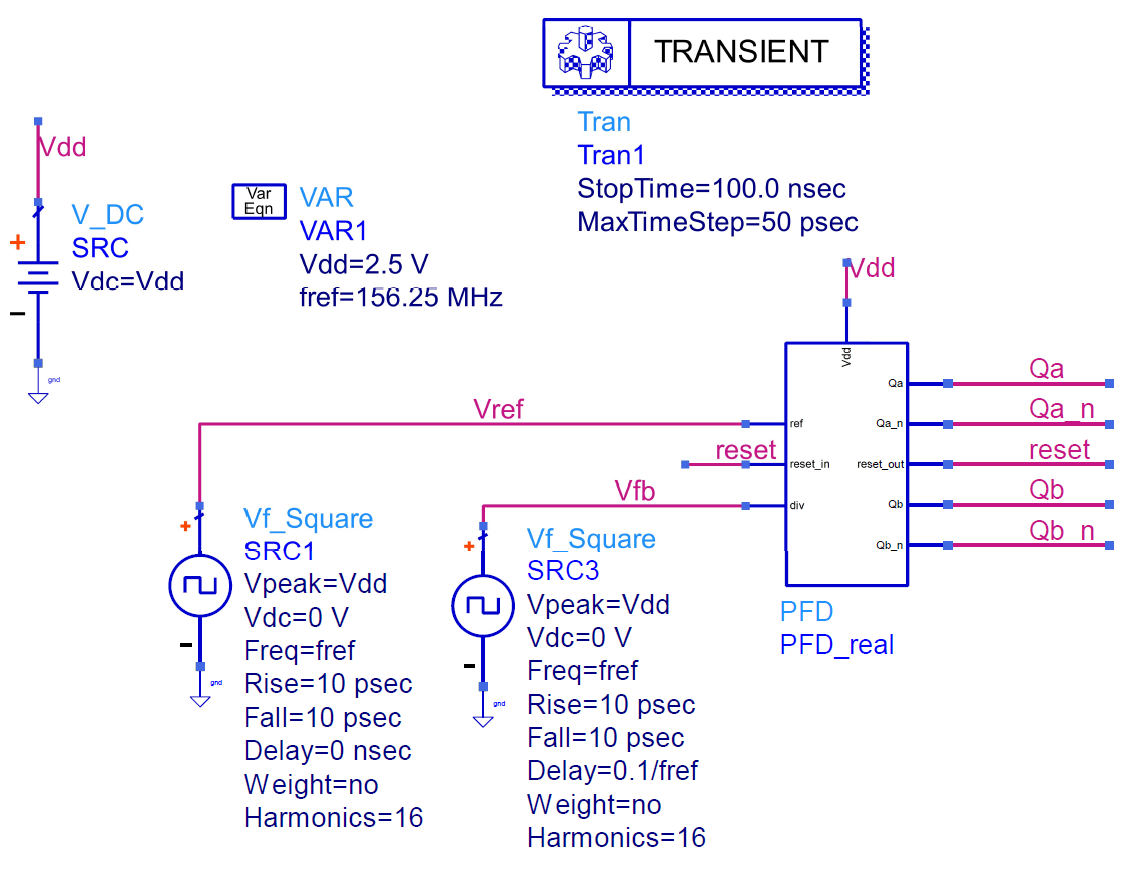
\includegraphics[width=1\linewidth]{images/block_design/PFD/pfd_test.png}
    \caption{PFD test schematic.}
    \label{fig:pfd_test}
\end{figure}

As shown in Fig.~\ref{fig:pfd_test_waveforms}, the output \( Q_a \) rises when a rising edge of the reference signal (\texttt{Vref}) is detected. Similarly, \( Q_b \) rises upon detection of a rising edge on the feedback signal (\texttt{Vfb}). This situation leads to a reset of the flip-flops, which occurs after a certain delay due to the propagation delay introduced by the AND gate. The opposite happens for negative phase delays (\texttt{Vfb} is early compared to \texttt{Vref}).

\begin{figure}[!ht]
    \centering
    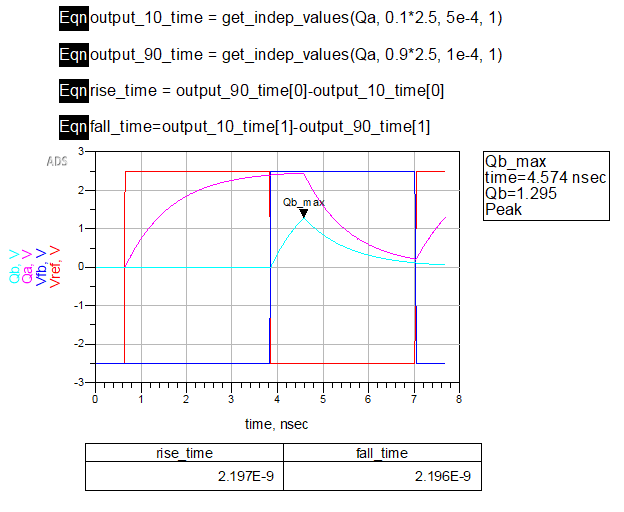
\includegraphics[width=1\linewidth]{images/block_design/PFD/pfd_test_measure.png}
    \caption{Dynamic characterization of the PFD outputs}
    \label{fig:pfd_dynamic}
\end{figure}

In Fig. \ref{fig:pfd_dynamic} a dynamic characterization of the PFD block has been carried out and the timing values have been reported in table \ref{tab:pfd_dynamic_values}.

\begin{table}[]
    \renewcommand{\arraystretch}{1.5}
    \centering
    \caption{Dynamic characterization of PFD outputs.}
    \label{tab:pfd_dynamic_values}
    \begin{tabular}{|c|c|c|}
    \hline
    $t_{rise}$ [\unit{\nano\second}] & $t_{fall}$ [\unit{\nano\second}] & Max spurious voltage [\unit{\volt}] \\ \hline
    2.197                   & 2.196                     & 1.295              \\ \hline
    \end{tabular}
\end{table}

As we can see, the outputs of the PFD using the ADS models for the D flip-flops and for the AND gate are characterized by a rise/fall time of about \SI{2.197}{\nano\second}: the bandwidth of the PFD is approximately $\frac{1}{\SI{2.197}{\nano\second}}\simeq\SI{455.2}{\mega\hertz}$, which, unfortunately, cannot be considered much higher than the input frequency $f_{ref}=\SI{156.25}{\mega\hertz}$. This means that particular attention must be paid to the CMOS implementation of these components, so that their frequency response will not represent a bottleneck for the whole PLL. Moreover, also the spurious peaks of $Q_b$ must be minimized by optimizing the propagation delay of the AND gate, in order to avoid unwanted activations of the charge pump stage.


\subsection{Charge Pump}
\label{sec:charge_pump}

\subsubsection{Design}
As anticipated before, the charge pump can source or sink a current, depending on its digital inputs from the phase-frequency detector, i.e. $Q_a$ (UP), $Q_b$ (DOWN) and their complementary digital values. A schematic view of a charge pump is shown in Fig. \ref{fig:cp_block_view}.

\begin{figure}[!ht]
    \centering
    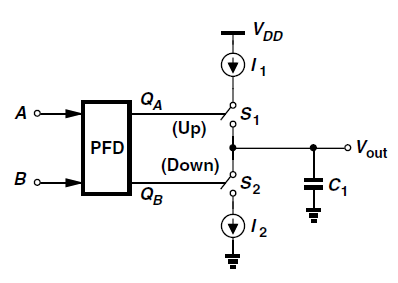
\includegraphics[width=1\linewidth]{images/block_design/CP/cp_block_view.png}
    \caption{Charge pump schematic view.}
    \label{fig:cp_block_view}
\end{figure}

The currents $I_1$ and $I_2$, also known as $I_{high}$ and $I_{low}$, are crucial in the design of the PLL dynamic response, given that the values of these currents represent the proportional gain of the loop and they can significantly affect its stability. In our design, we chose $I_{high}=I_{low}=I_{CP}=\qty{400}{\micro\ampere}$: this value was chosen to ensure a high DC open loop gain and so that the overdrive voltage of current reference MOSFETs is high enough to guarantee that their bias is in the saturation region.

Many different charge pump implementations exist in scientific literature. The architecture chosen in this design is a \textbf{drain switching} with \textbf{improved matching}, presented in Fig. \ref{fig:cp-architecture}.

\begin{figure}[!ht]
    \centering
    \def\svgwidth{\linewidth}
    \input{images/block_design/CP/cp_schematic.pdf_tex}
    \caption{Architecture of a drain switching charge pump with improved matching.}
    \label{fig:cp-architecture}
\end{figure}

The unity gain amplifier is used to compensate for the mismatch between the upper and the lower currents, which would cause a significant phase error.

The implementation using the \qty{0.25}{\micro\meter} technology made in ADS is illustrated in Fig. \ref{fig:cp_ads_schematic}. The power supply voltage is set to $V_{DD}=\qty{2.5}{\volt}$

\begin{figure}[!ht]
    \centering
    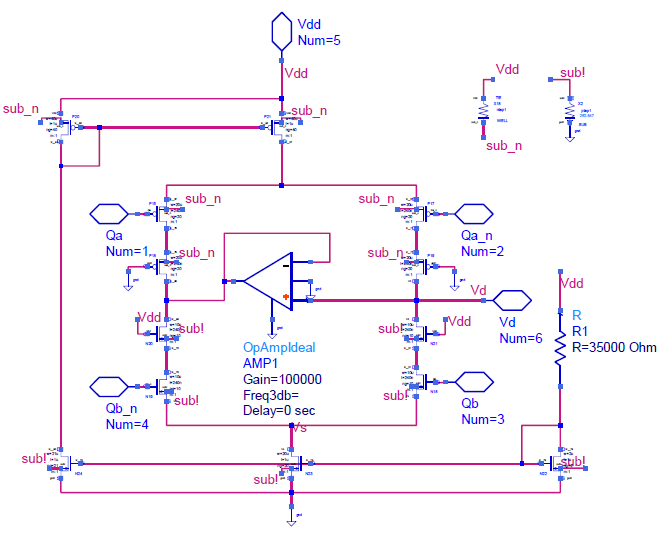
\includegraphics[width=1.0\linewidth]{images/block_design/CP/cp_schematic_ads.png}
    \caption{ADS charge pump schematic.}
    \label{fig:cp_ads_schematic}
\end{figure}

Here we can see that the pMOS and nMOS attached to the four digital input terminals ($M_6,\ M_7,\ M_{12}\text{ and }M_{13}$) are the actual switches of the charge pump, whereas the other four MOSFETs in series with the switches ($M_8,\ M_9,\ M_{10}\text{ and }M_{11}$) are used to increase the output impedance of the device and they are always turned on. The transistor in the top ($M_4,\ M_5$) and bottom ($M_1,\ M_2 \text{ and } M_3$) tails are the current mirrors that set the \(I_{high}\) and \(I_{low}\) currents at \qty{400}{\micro\ampere}.

The MOSFETs dimensions were designed considering the SG25H4 process parameters for long channel nMOS and pMOS: electron mobility \(\mu_n=\qty[per-mode=symbol]{0.032}{\volt\second\per\meter}\), symmetrical threshold voltages \(V_{tn}=-V_{tp}=\qty{0.6}{\volt}\) and oxide capacitance density \(C_{ox}=\qty[per-mode=symbol]{5.31}{\milli\farad\per\meter}\). The MOSFETs of the top and bottom current mirrors were designed with a channel length \(L=\qty{1}{\micro\meter}\) four times greater than the minimum allowed by this technology, in order to be able to neglect channel length modulation effects. The master of the bottom mirror ($M_1$) was designed to be biased at an overdrive voltage of \(V_{GS}-V_{t}=\qty{500}{\milli\volt}\) with a current \(I_{bias}=\qty{40}{\micro\ampere}\), therefore, the current expression for a long channel MOSFET

\begin{equation}\label{eq:long_channel_current}
    I_D = \frac{\mu_nC_{ox}}{2}\frac{W}{L}\left(V_{GS}-V_{t}\right)^2
\end{equation}

we were able to calculate the ratio between width and length \(\frac{W}{L}=1.88\). A width of \qty{2}{\micro\meter} was chosen. Given the overdrive voltage, the gate-source voltage is \(V_{GS}=V_{t}+\qty{500}{\milli\volt}=\qty{1.1}{\volt}\) and the bias resistance can be obtained as follows:

\begin{equation}\label{eq:r_bias}
    R_{bias}=\frac{V_{dd}-V_{GS}}{I_{bias}}=\qty{35}{\kilo\ohm}
\end{equation}

All the other MOSFETs that compose the top and bottom mirrors can be designed considering that the required current amplification factor is \(\frac{I_{CP}}{I_{bias}}=\frac{\qty{400}{\micro\ampere}}{\qty{400}{\micro\ampere}}=10\): using the same length of \qty{1}{\micro\meter}, the widths of the type n MOSFETs are set to be 10 times greater than the width of the bias MOSFET (\(W=\qty{20}{\micro\meter}\)), whereas this value has to be doubled for the p type MOSFETs, in order to compensate for the fact that the mobility of holes is \(\mu_p\simeq\frac{\mu_n}{2}\).

The switching and dummy MOSFETs were designed to have a behavior similar to ideal switches. Their lengths were set to the minimum allowed by this technology (\qty{0.24}{\micro\meter} this allows for faster switching rates) and their widths were set to \qty{10}{\micro\meter} for nMOS and to \qty{20}{\micro\meter} for pMOS. This way their \(\frac{W}{L}\) ratio is doubled compared to the one used in the current mirror transistors and, when turned on, they will be forced to work in the triode region, with small \(V_{DS}\) and high conductivity.

\begin{figure*}[!ht]
    \centering
    \subfloat[]{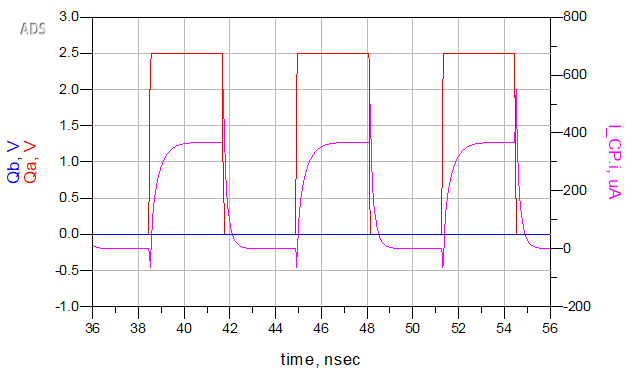
\includegraphics[width=0.5\linewidth]{images/block_design/CP/cp_currents_up_50.png}%
    \label{fig:currents_up_50}}
    \hfil
    \subfloat[]{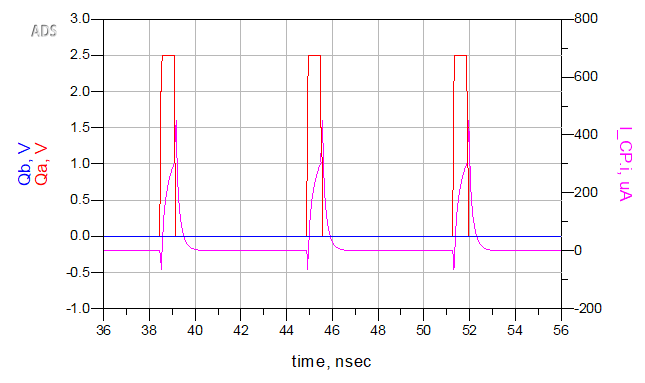
\includegraphics[width=0.5\linewidth]{images/block_design/CP/cp_currents_up_10.png}%
    \label{fig:currents_up_10}}
    \hfil
    \subfloat[]{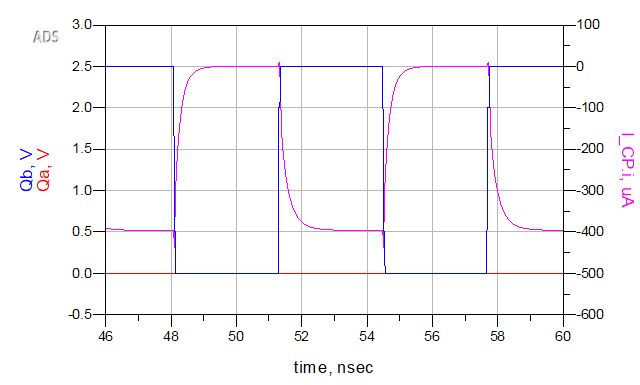
\includegraphics[width=0.5\linewidth]{images/block_design/CP/cp_currents_down_50.png}%
    \label{fig:currents_down_50}}
    \hfil
    \subfloat[]{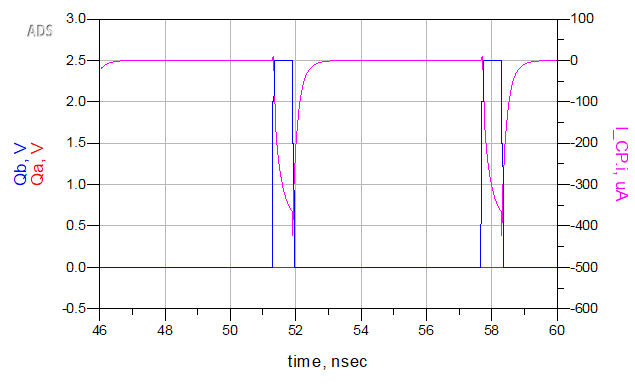
\includegraphics[width=0.5\linewidth]{images/block_design/CP/cp_currents_down_10.png}%
    \label{fig:currents_down_10}}
    \hfil
    \caption{Charge pump currents: (a) and (b) show source currents (\(Q_a\) high) for different values of delay time (\(\frac{0.5}{f_{ref}}\) and \(\frac{0.1}{f_{ref}}\) respectively); (c) and (d) show sink currents (\(Q_b\) high) for diffrent values of delay time (\(\frac{0.5}{f_{ref}}\) and \(\frac{0.1}{f_{ref}}\) respectively)} 
    \label{fig:cp_test_waveforms}
\end{figure*}

In table \ref{tab:cp_mos_size}, a summary of the used sizes of the charge pump MOSFETs is shown. For all MOSFETs, their multiplier is set to 1.

\begin{table}[!ht]
    \renewcommand{\arraystretch}{1.5}
    \centering
    \caption{Charge Pump MOSFETs dimensions}
    \label{tab:cp_mos_size}
    \begin{tabular}{|c|c|c|c|}
    \hline
    \textbf{L \([\mu m]\)} & \textbf{W \([\mu m]\)} & \textbf{Number of gates} & \textbf{Devices} \\ \hline
    1               & 2              & 2                        & $M_1$                  \\ \hline
    1               & 20             & 20                       & $M_2,\ M_3$                 \\ \hline
    1               & 40             & 40                       & $M_4,\ M_5$                 \\ \hline
    0.24            & 10             & 10                       & $M_6,\ M_7,\ M_8,\ M_9$                   \\ \hline
    0.24            & 20             & 20                       & $M_{10},\ M_{11},\ M_{12},\ M_{13}$                 \\ \hline
    \end{tabular}
\end{table}

The unity gain operational amplifier has been modeled using the ideal component found in the ADS library, using a differential open loop gain of 100 dB.

It is worth noting that the SG25H4 library offers two nMOSFET models, the \texttt{nmos} and the \texttt{rfnmos}, where the latter differs from the former for some layout considerations and for its special RF model. However, in the case of this charge pump the \texttt{nmos} model was used, given that this device will be used at relatively low frequencies (156.25 MHz). 

\subsubsection{Test}
\begin{figure*}[!ht]
    \centering
    \subfloat[]{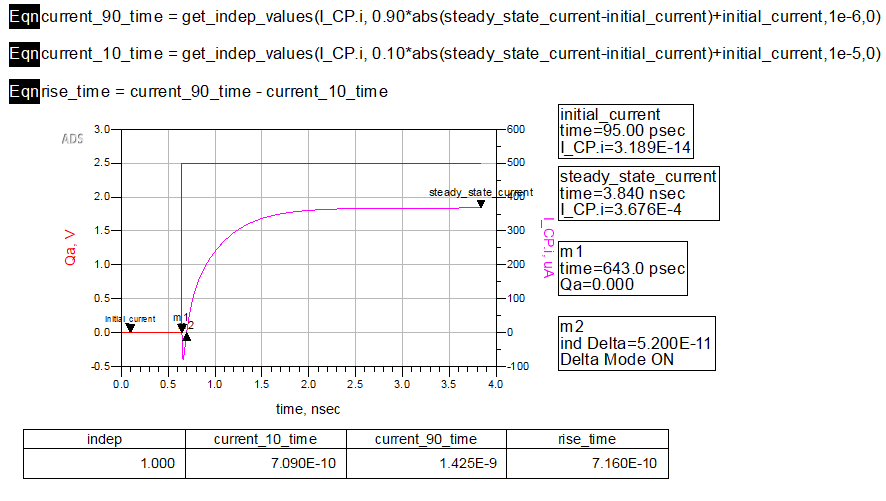
\includegraphics[width=0.5\linewidth]{images/block_design/CP/up_rising_current_test.png}%
    \label{fig:up_rising}}
    \hfil
    \subfloat[]{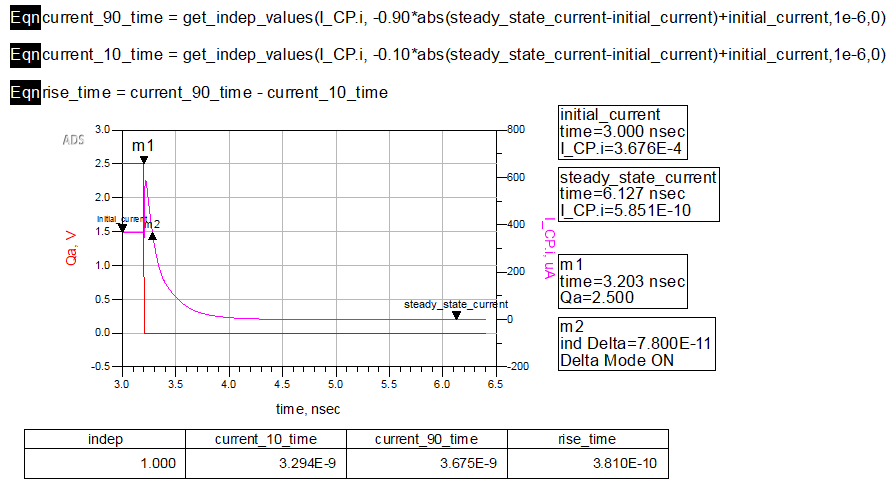
\includegraphics[width=0.5\linewidth]{images/block_design/CP/up_falling_current_test.png}%
    \label{fig:up_falling}}
    \hfil
    \subfloat[]{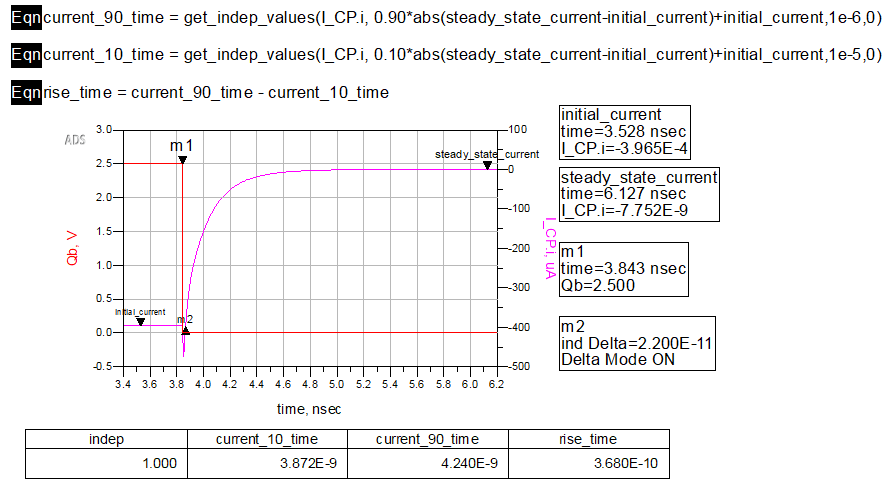
\includegraphics[width=0.5\linewidth]{images/block_design/CP/down_falling_current_test.png}%
    \label{fig:down_rising}}
    \hfil
    \subfloat[]{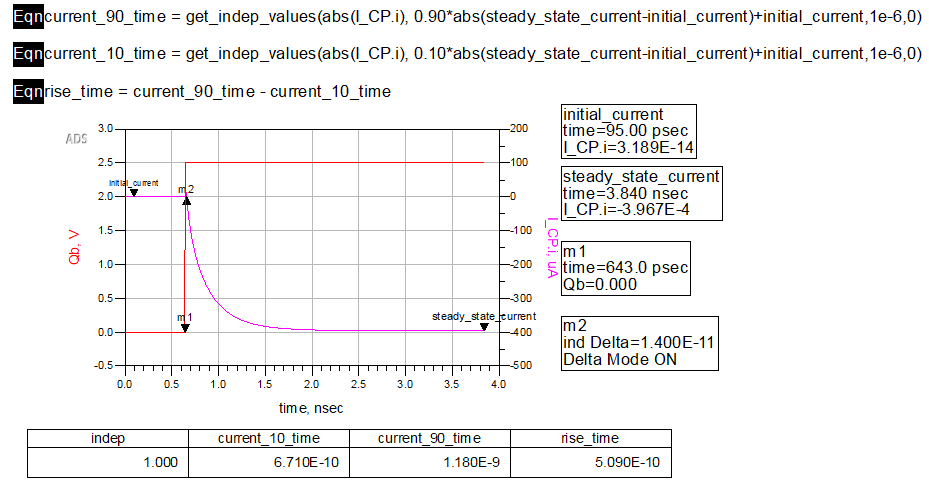
\includegraphics[width=0.5\linewidth]{images/block_design/CP/down_rising_current_test.png}%
    \label{fig:down_falling}}
    \hfil
    \caption{Dynamic characterization of charge pump output values for rising and falling edges of the source current ((a), (b)) and for rising and falling edges of the sink current ((c), (d)).} 
    \label{fig:dynamic_spec_cp_currents}
\end{figure*}

The charge pump cell was tested in ADS generating realistic inputs using the ideal model of a phase-frequency detector, already present in the library. The inputs for the PFD were connected to two ideal square waves at a frequency of 156.25 MHz (\(f_{ref}\)) and with a variable phase delay between the two. The testbench used is shown in Fig. \ref{fig:cp_testbench_schematic}.

\begin{figure}[!ht]
    \centering
    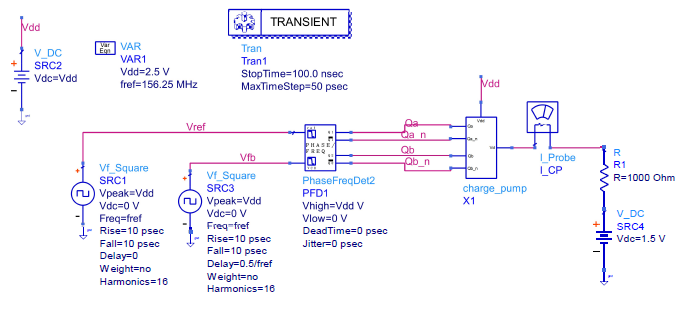
\includegraphics[width=1\linewidth]{images/block_design/CP/cp_test_schematic.png}
    \caption{Charge pump testbench in ADS.}
    \label{fig:cp_testbench_schematic}
\end{figure}

Notice the presence of a constant voltage at the output of the charge pump cell: this is necessary in order to allow a correct polarization of the tail mirror during the sink current test; otherwise, the \(V_{DS}\) of the bottom tail would be 0 V and no current could be sunk.

Performing a transient simulation, both with \texttt{Vfb} delayed compared \texttt{Vref} (\(Q_a\) is high) and viceversa (\(Q_b\) is high), the current waveforms in Fig. \ref{fig:cp_test_waveforms} were measured on the load.

Considering the tests made with half of a period of delay between the input signals (\(\frac{0.5}{f_{ref}}\)), we coul evaluate the dynamic characteristics of the designed charge pump. In particular, as shown in Fig. \ref{fig:dynamic_spec_cp_currents} we measured the delay time of the currents and the rise/fall times (from 10\% to 90\% of the steady-state current value). The final delay time is evaluated as the average between the delay time before a rising edge and before a falling edge. The results found are listed in table \ref{tab:cp_dynamic_values}.

\begin{table}[]
    \renewcommand{\arraystretch}{1.5}
    \centering
    \caption{Dynamic characterization of charge pump output currents.}
    \label{tab:cp_dynamic_values}
    \begin{tabular}{|c|c|c|c|c|}
    \hline
    Current type & $I\ [\mu A]$ & $t_{delay}\  [ps]$ & $t_{rise} [ps]$ & $t_{fall}\ [ps]$ \\ \hline
    Source                   & 367.6                     & 65                    & 716         & 381              \\ \hline
    Sink                     & -396.7                     & 18                    & 509         & 368              \\ \hline
    \end{tabular}
\end{table}

As we can see, the worst-case rise time is 716 ps, which corresponds to a bandwidth of the charge pump of \(\frac{1}{\SI{716e-12}{\second}}\simeq\SI{1.4}{\giga\hertz}\), approximately 10 times the input frequency \(f_{ref}=\SI{156.25}{\mega\hertz}\). Therefore, we can neglect the effects of the charge pump on the closed-loop bandwith of the PLL system.

On the other hand, we can see an inevitable mismatch between the source and sink currents: as explained in \cite{razavi_current_mismatch}, the PLL system will develop a phase offset such that the smaller current lasts longer.

\subsection{Voltage Controlled Oscillator and Frequency Divider}\label{sec:vco}
The used VCO (Voltage Controlled Oscillator) used in the model of our PLL is an ideal ADS library component, noiseless and with no lock limitation, whose symbol is shown in Fig. \ref{fig:vco_symbol}.

\begin{figure}[!ht]
    \centering
    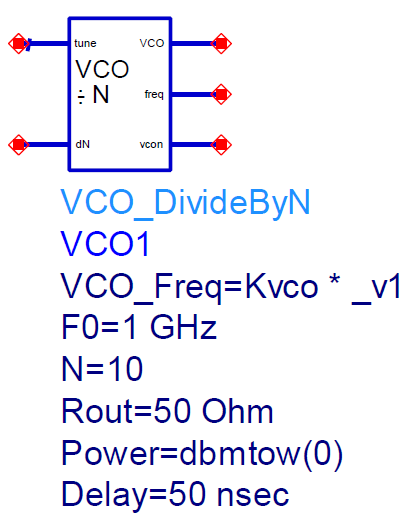
\includegraphics[width=0.5\linewidth]{images/block_design/VCO/vco_symbol.png}
    \caption{Ideal VCO with FD from ADS library.}
    \label{fig:vco_symbol}
\end{figure}

It also implements a FD (Frequency Divider) and presents at one of its output terminal the frequency of the VCO divided by the parameter \texttt{N}: for simulation purposes - as explained in the ADS Help manual - this divided output will be a sawtooth waveform, whose open circuit voltage represents the istantaneous phase, in radians, of the divided signal. Therefore this sawtooth waveform will span in the range \(\left[-\pi,\pi\right]\), with an istantaneous slope of

\begin{equation}\label{eq:sawtooth_slope}
    S_{sawtooth}=2\pi \frac{f_{VCO}(t)}{N}+\theta(t)
\end{equation}

It is trivial to prove that the istantaneous period of this sawtooth changes with the VCO frequency and will be equal to \(\frac{N}{f_{VCO}(t)}\). The istantaneous variation of frequency of the VCO \(\Delta f(t)\) from its central frequency \(f_0\) is proportional to the voltage input at the terminal \texttt{tune}, following this relationship:

\begin{equation}\label{eq:vco_freq}
    \Delta f(t) = K_{VCO}\cdot v_{tune}(t)
\end{equation}

The total VCO frequency is given at the \texttt{freq} output terminal, whose open circuit voltage is the istantaneous VCO frequency \(f_{VCO}(t)=f_0+\Delta f(t)\) expressed in GHz.

For our simulations purposes, we chose to use the parameters of the 65 nm LC-tank VCO for SpaceFibre applications designed at the University of Pisa \cite{vco}, even though implemented in a different technology compared to ours. Therefore, we set \(K_{VCO}=2\ \frac{GHz}{V}\) and \(f_0=5.95\ GHz\).



\section{ADS Simulations}
\label{sec:ADS_simulations}
In this section, the implementation and simulations performed in ADS are presented. 

First, an ideal charge pump PLL using behavioral models is shown. Subsequently, the PFD, CP, and loop filter are replaced with the designed blocks described in Section~\ref{sec:block_design}. The system's response to frequency and phase steps is also analyzed. Finally, a section is dedicated to phase noise evaluation, which is performed using behavioral models.

\subsection{Ideal system simulation}

\begin{figure*}[!ht]
    \centering
    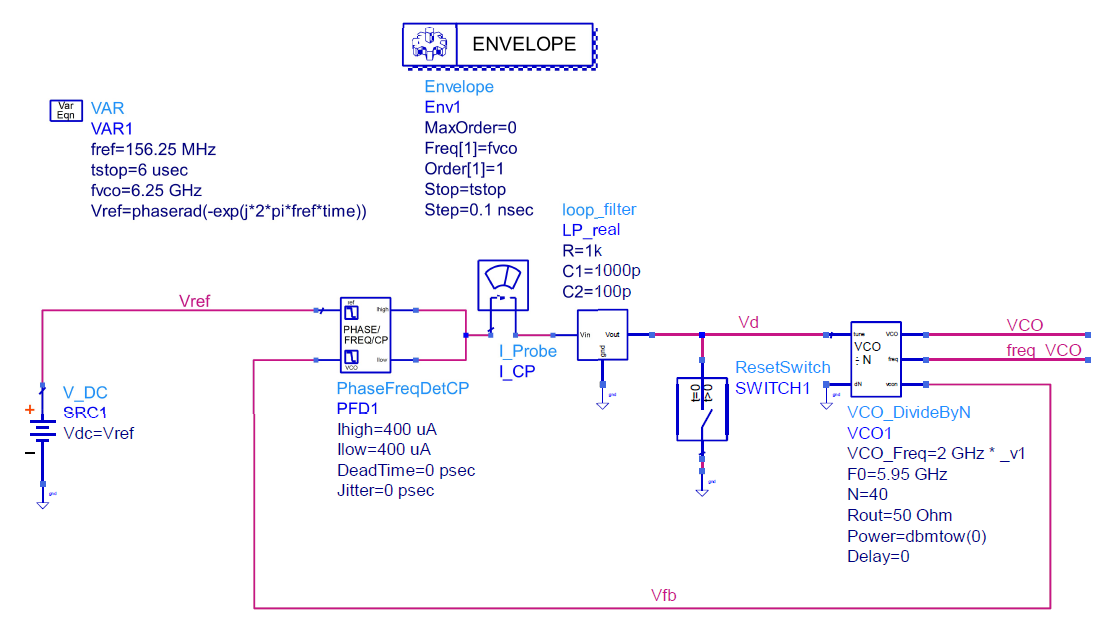
\includegraphics[width=0.7\linewidth]{images/intro_system_level/pll_ideal.png}
    \caption{CP-PLL ideal.}
    \label{fig:PLL_ideal}
\end{figure*}

Figure~\ref{fig:PLL_ideal} shows the PLL system implemented using ADS library blocks. This system is simulated using an envelope simulation, a technique that significantly reduces simulation time. The envelope simulation combines transient simulation for baseband signals and harmonic balance for narrowband signals near the carrier frequency. 

This type of simulation is feasible because behavioral models are utilized. In this approach, both the output frequency of the VCO and the input signals of the PFD-CP are represented as sawtooth waveforms, as already explained in Section\ref{sec:vco}. These signals depict the instantaneous frequency rather than the entire waveform, simplifying the simulator's task of identifying rising edges and improving computational efficiency.

To ensure compatibility with the envelope simulation approach, the reference frequency (\(f_{\text{ref}}\)) is also represented in the form of a phase. This is achieved using the expression:

\[
V_{\text{ref}} = \text{phaserad}\left(-\exp(j \cdot 2\pi \cdot f_{\text{ref}} \cdot \text{time})\right),
\]

where \texttt{phaserad} returns the phase in radians of the expression within the parentheses, which involves a complex exponential. 

Moreover, to better emulate a realistic scenario, a switch is included between the loop filter and the VCO. This allows the system to replicate an actual startup condition, providing insight into the transient behavior during lock acquisition.

\begin{figure*}[!ht]
    \centering
    \subfloat[]{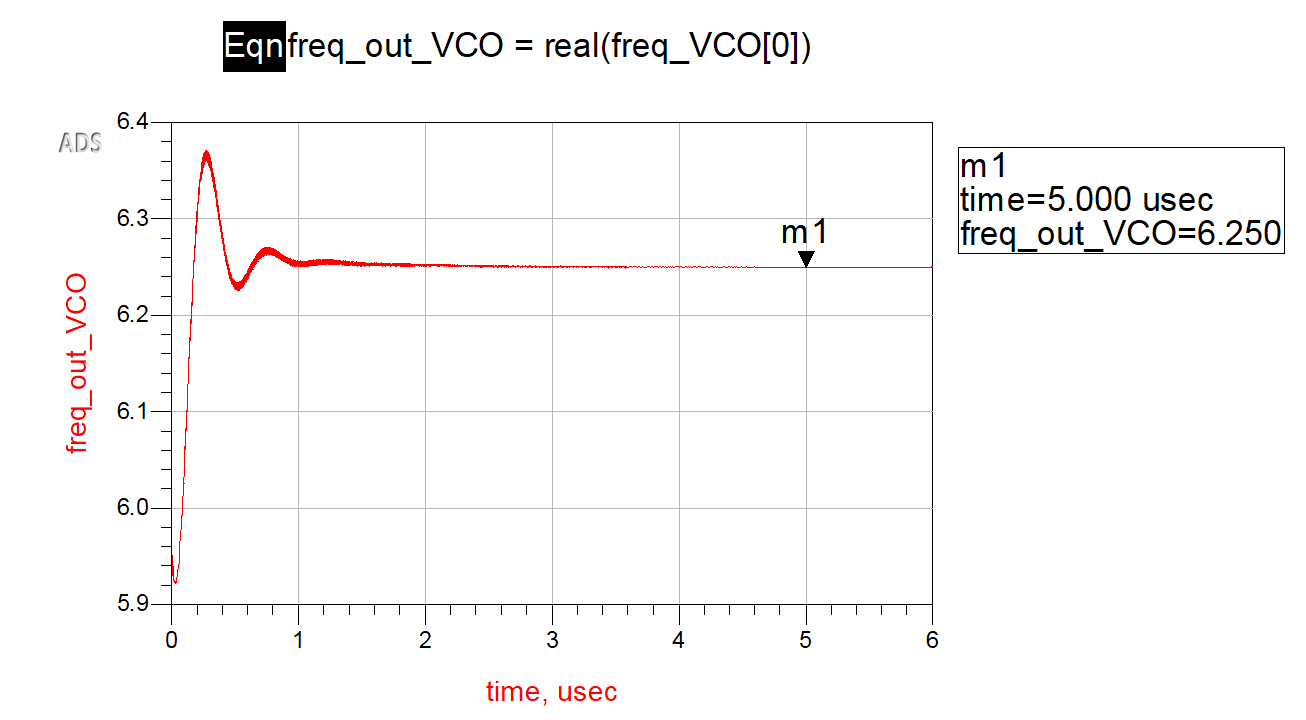
\includegraphics[width=0.5\linewidth]{images/ads_results/ideal_pll/freq_VCO_ideal.png}%
    \label{fig:freq_VCO_ideal}}
    \hfil
    \subfloat[]{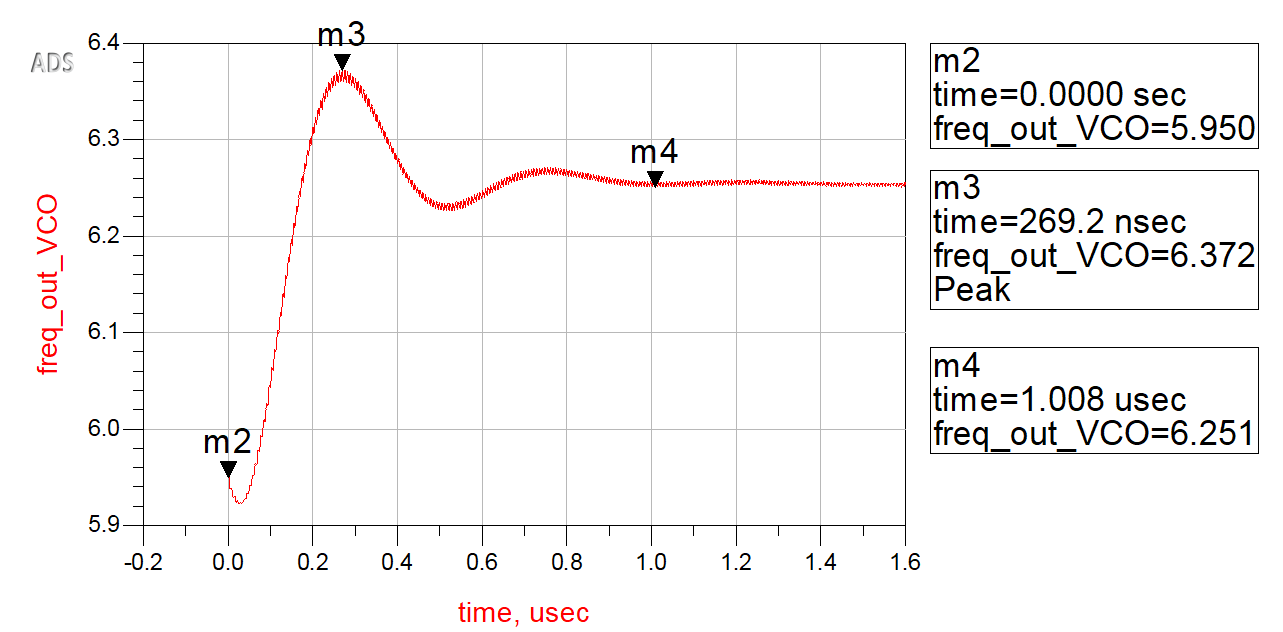
\includegraphics[width=0.5\linewidth]{images/ads_results/ideal_pll/freq_VCO_ideal_zoom.png}%
    \label{fig:freq_VCO_ideal_zoomed}}
    \hfil
    \subfloat[]{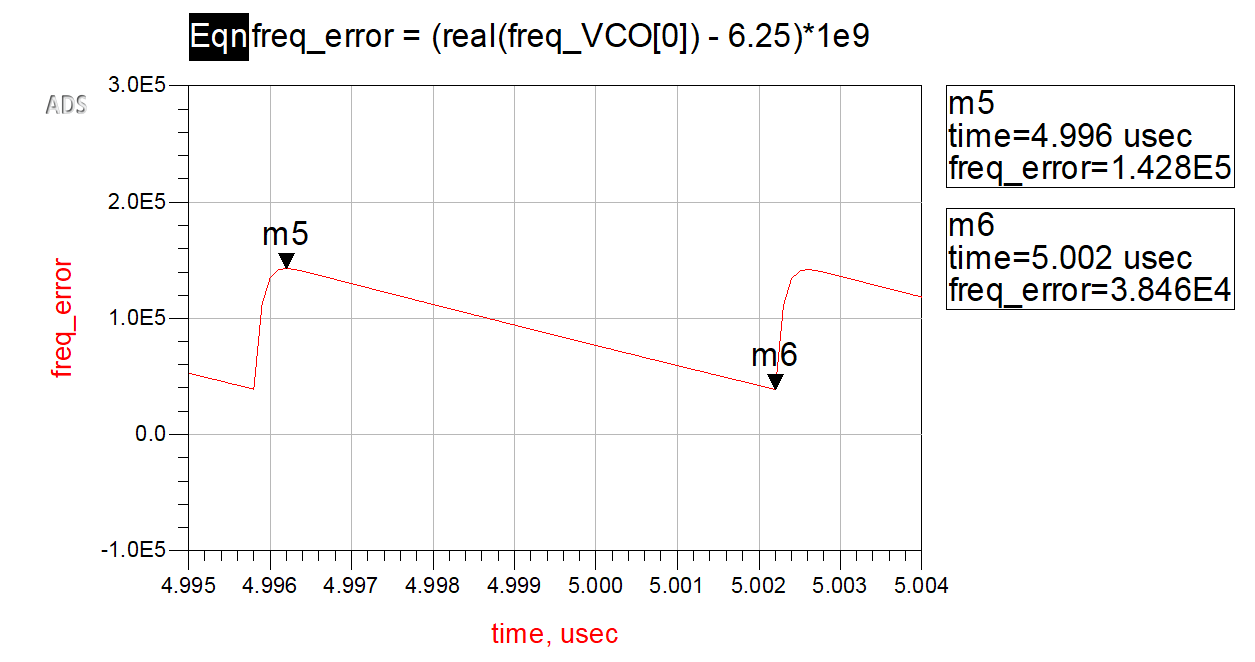
\includegraphics[width=0.5\linewidth]{images/ads_results/ideal_pll/freq_error_VCO_ideal.png}%
    \label{fig:freq_error_VCO_ideal}}
    \hfil
    \subfloat[]{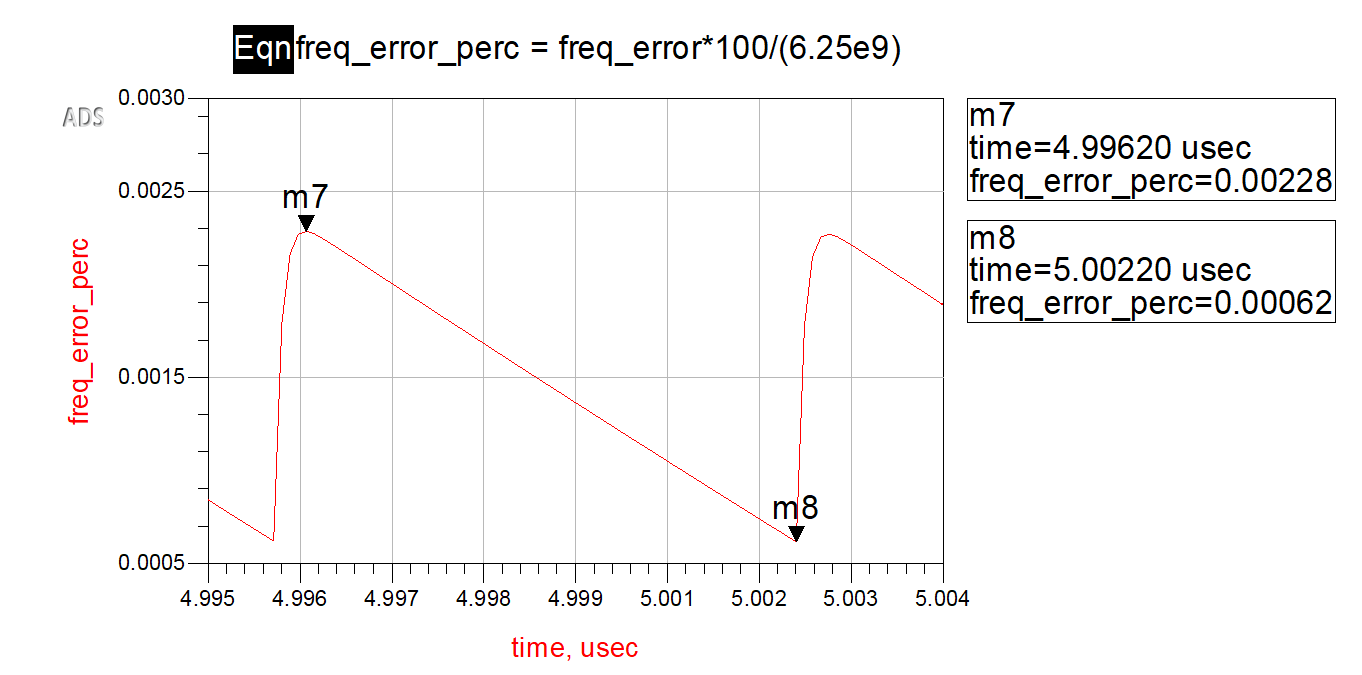
\includegraphics[width=0.5\linewidth]{images/ads_results/ideal_pll/freq_error_perc_VCO_ideal.png}%
    \label{fig:freq_error_perc_VCO_ideal}}
    \hfil
    \caption{Ideal simulation: (a) Frequency output over time, (b) Frequency over time zoomed, (c) Frequency output error over time, (d) Frequency output error percentage over time.}
    \label{fig:freq_VCO_ideal_and_zoomed}
\end{figure*}

In Fig.~\ref{fig:freq_VCO_ideal_and_zoomed}, the output frequency of the closed-loop system is shown. As can be observed, the PLL achieves lock after approximately \(1 \, \mu\text{s}\), stabilizing the output at \(6.25 \, \text{GHz}\). The result is obtained by plotting the baseband output frequency of the VCO, which is one of the possible types of plots available in the envelope simulation.

From Fig.~\ref{fig:freq_VCO_ideal_zoomed}, it is also possible to observe a zoomed view of the transient behavior of the output frequency. Initially, the VCO output starts at \(5.95 \, \text{GHz}\), as expected. It then exhibits an overshoot, reaching \(6.372 \, \text{GHz}\) after \(269.2 \, \text{ns}\), before stabilizing at \(6.25 \, \text{GHz}\) after \(1 \, \mu\text{s}\), due to the second-order loop filter, which is characteristic of the chosen design.

For a more detailed analysis of the dynamic response of the designed PLL, it is more informative to examine the figure of merit after a frequency step during steady-state operation, as will be discussed in Section~\ref{sec:freq_step}.  

A frequency error ranging from \(38.46 \, \text{kHz}\) to \(142.8 \, \text{kHz}\) is obtained, which corresponds to a percentage error ranging from \(0.00228 \, \%\) to \(0.00062 \, \%\). This demonstrates the high precision of the designed PLL system. The frequency error and its behavior over time are shown in Fig.~\ref{fig:freq_VCO_ideal_and_zoomed}.

\begin{figure}[!ht]
    \centering
    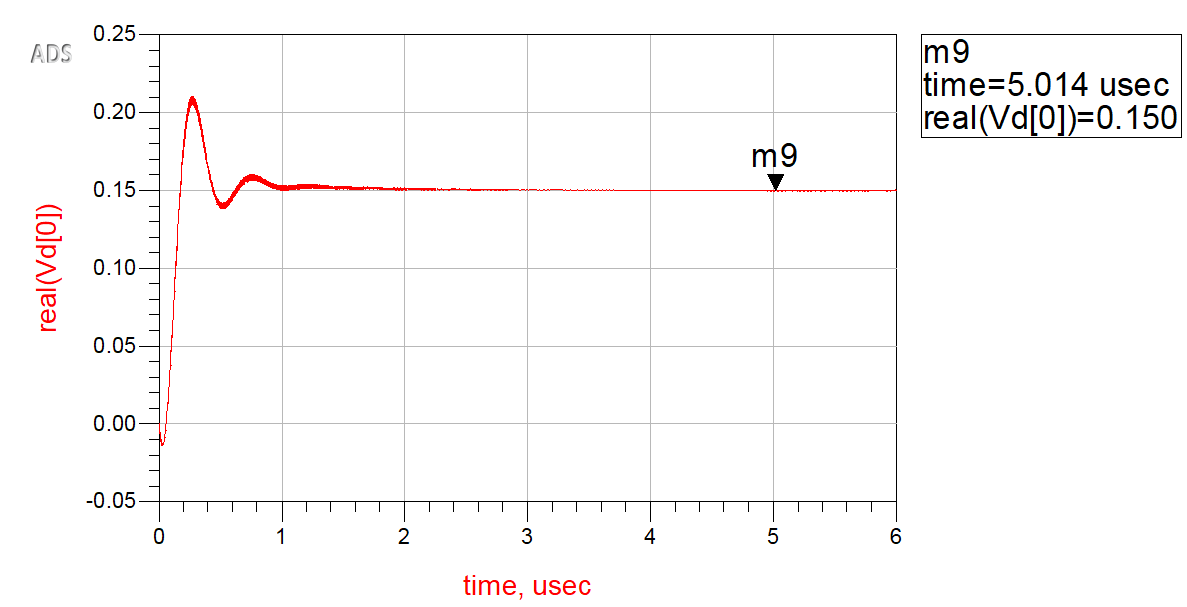
\includegraphics[width=1\linewidth]{images/ads_results/ideal_pll/Vd_ideal.png}
    \caption{Ideal simulation: Control voltage over time.}
    \label{fig:Vd_ideal}
\end{figure}

In Fig.~\ref{fig:Vd_ideal}, the control voltage for the VCO (\(V_d\)) is shown. It illustrates the ideal characteristics of the VCO used, where the instantaneous output frequency is proportional to \(V_d\) by the sensitivity factor (\(K_{VCO}\)). The steady-state value of \(V_d\) is \(0.15 \, \text{V}\), consistent with the predicted behavior. 

The VCO is modeled by the equation 
\[
V_d \cdot K_{VCO} = \theta \cdot s
\] 
in the Laplace domain, indicating that the control voltage is proportional to the instantaneous variation of frequency. Given \(K_{VCO} = 2 \, \text{GHz/V}\) and a starting frequency of \(5.95 \, \text{GHz}\), the output frequency can be calculated as follows:
\[
0.15 \cdot 2 \times 10^9 + 5.95 \times 10^9 = 6.25 \times 10^9 \, \text{Hz}
\]
This confirms the expected steady-state frequency of \(6.25 \, \text{GHz}\).


\begin{figure}[!h]
    \centering
    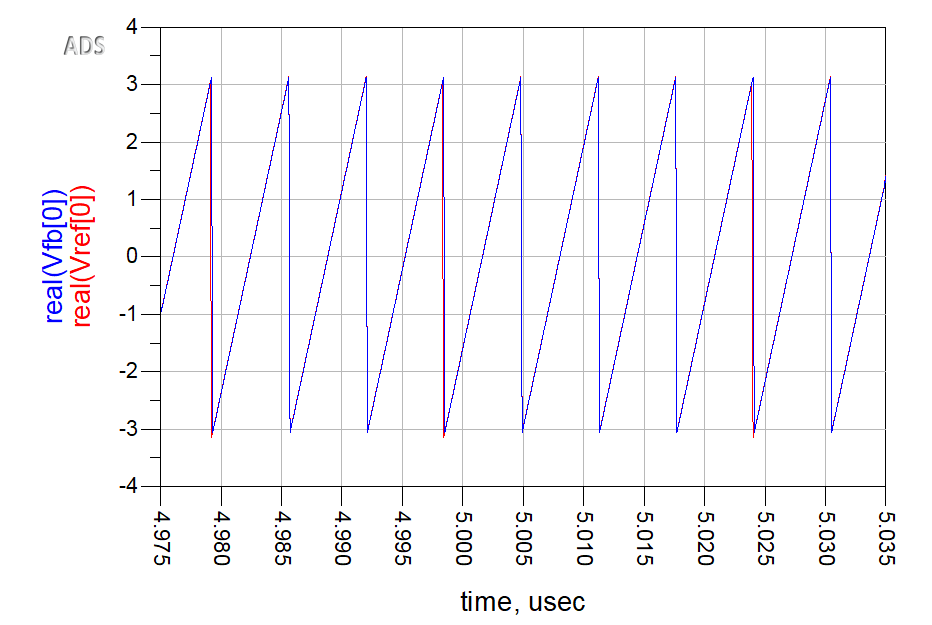
\includegraphics[width=1\linewidth]{images/ads_results/ideal_pll/Vref_Vfb_idea.png}
    \caption{Ideal simulation: Reference and Feedback signals over time.}
    \label{fig:Vref_Vfb_ideal}
\end{figure}

Finally, the inputs of the phase-frequency detector are compared in Fig.~\ref{fig:Vref_Vfb_ideal}, where the overlapping of the signals can be observed. Thus, we can conclude that the ideal PLL not only achieves the desired output frequency but also maintains phase alignment with the reference frequency.

\subsection{Real system simulation}

\begin{figure*}[!hb]
    \centering
    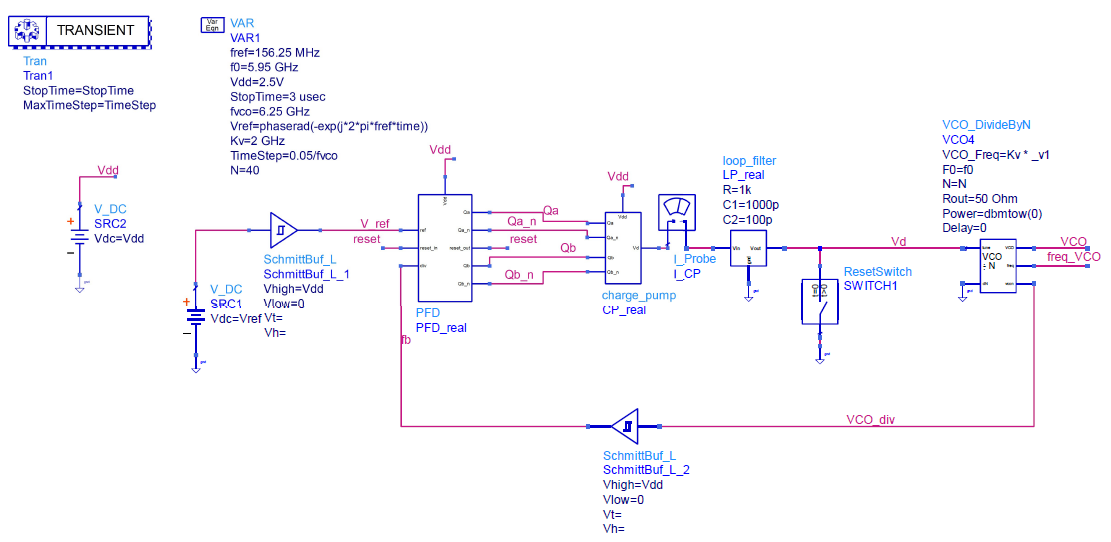
\includegraphics[width=0.75\linewidth]{images/ads_results/real_pll/pll_real.png}
    \caption{CP-PLL real.}
    \label{fig:PLL_real}
\end{figure*}

In Fig.~\ref{fig:PLL_real}, the ADS implementation of the entire system is shown. First of all, it is important to note that the simulation must be performed using a transient analysis. This is because the flip-flops used in the PFD cannot detect the crossing points of continuous signals and, therefore, cannot be triggered using an envelope-type simulation. 

To ensure compatibility with the behavioral model of the VCO, two ideal Schmitt triggers are employed to generate impulse signals as inputs to the PFD. The sawtooth wave signal provided by the VCO (\texttt{VCO\_div}) is a periodic signal with a time period \(T = 1 / f_{\text{ref}}\). Thus, an ideal comparator suffices to produce inputs compatible with the flip-flops in the PFD. 

The \texttt{SchmittBuf\_L} block, provided by the ADS library, is used as an ideal Schmitt trigger in this work. All its parameters are left at their default values since they are necessary only for simulation purposes. This simulation is particularly insightful for analyzing the differences compared to the ideal schematic, including details in the output spectrum.

It is important to note that this simulation is performed without any phase noise, which will be addressed in Section~\ref{sec:phase_noise}. Therefore, the results and conclusions should be interpreted under ideal conditions.

\begin{figure}[!ht]
    \centering
    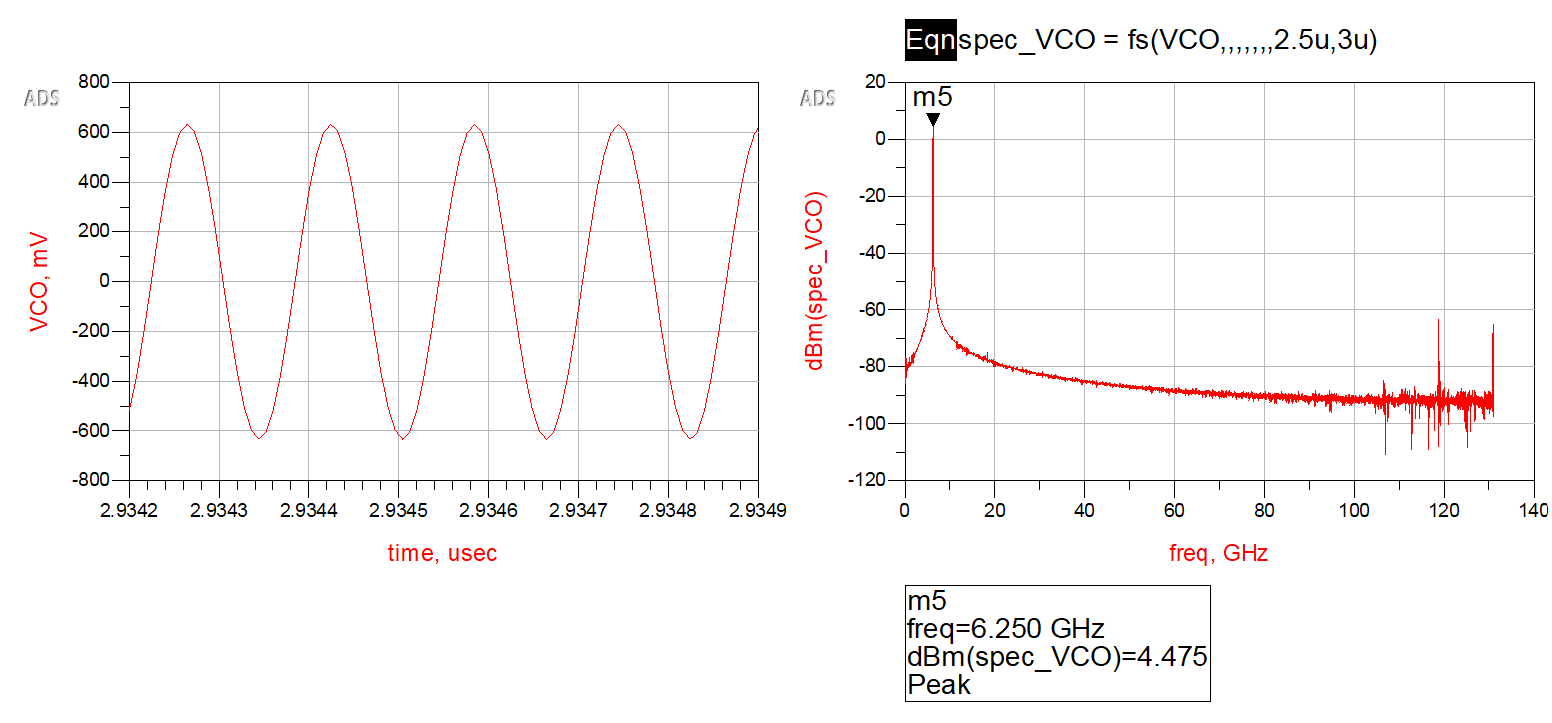
\includegraphics[width=1\linewidth]{images/ads_results/real_pll/vco_out_real_results.png}
    \caption{Real simulation: VCO output voltage and VCO output spectrum.}
    \label{fig:vco_out_real_results}
\end{figure}

First of all, in Fig.~\ref{fig:vco_out_real_results}, the output sinusoidal signal of the VCO and its corresponding spectrum are shown. The spectrum is obtained using the built-in \texttt{fs()} function in ADS, focusing on a reduced time period during steady-state conditions. This approach ensures that the spectrum reflects only the steady-state behavior, excluding dynamic spurious components. As observed, a prominent peak is present at \(6.25 \, \text{GHz}\), as expected.

Moreover, in Fig.~\ref{fig:freq_VCO_real_and_zoom}, the same plots are presented as those for the ideal PLL. In this case, the overshoot occurs after \(251.5 \, \text{ns}\), reaching a value of \(6.369 \, \text{GHz}\). The steady-state regime is achieved in approximately the same time as the ideal case, around \(1 \, \mu\text{s}\). 

The frequency error exhibits a maximum of \(227.5 \, \text{kHz}\) and a minimum of \(1.524 \, \text{kHz}\), corresponding to percentage errors of \(0.00364 \, \%\) and \(0.00002 \, \%\), respectively. These results further demonstrate the high precision of the designed PLL system, even when considering the real implementation.

\begin{figure*}[!ht]
    \centering
    \subfloat[]{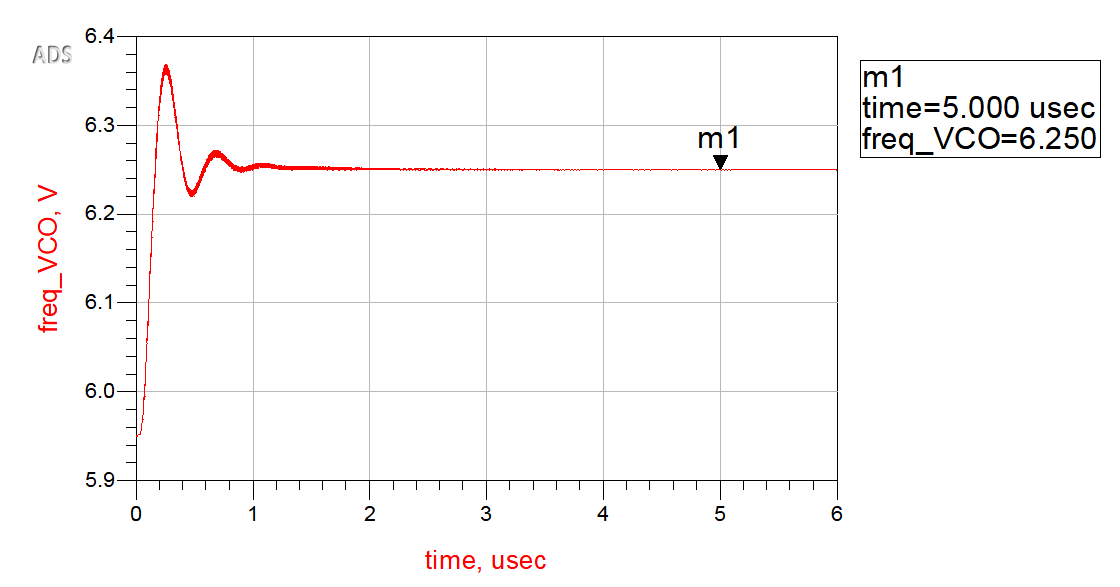
\includegraphics[width=0.5\linewidth]{images/ads_results/real_pll/freq_VCO_real.png}%
    \label{fig:freq_VCO_real}}
    \hfil
    \subfloat[]{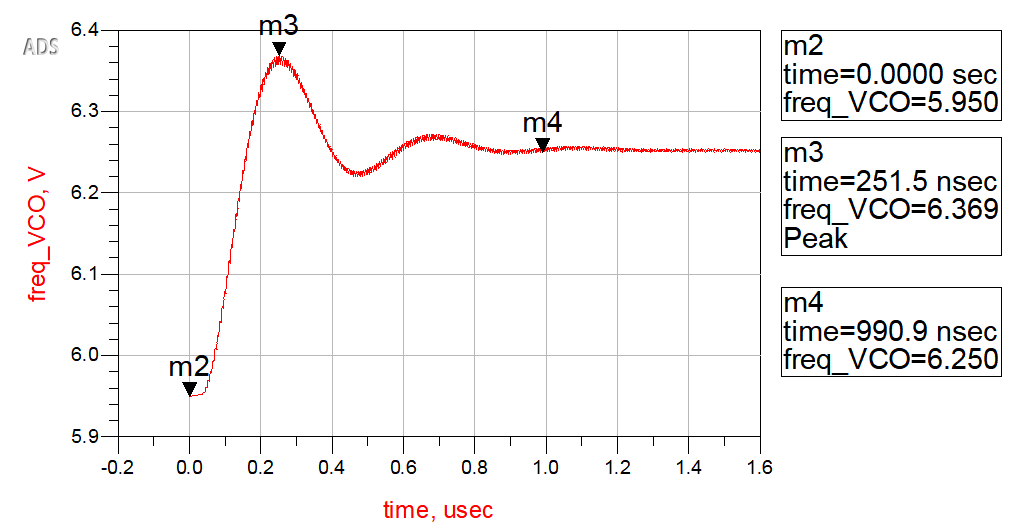
\includegraphics[width=0.5\linewidth]{images/ads_results/real_pll/freq_VCO_real_zoom.png}%
    \label{fig:freq_VCO_real_zoom}}
    \hfil
    \subfloat[]{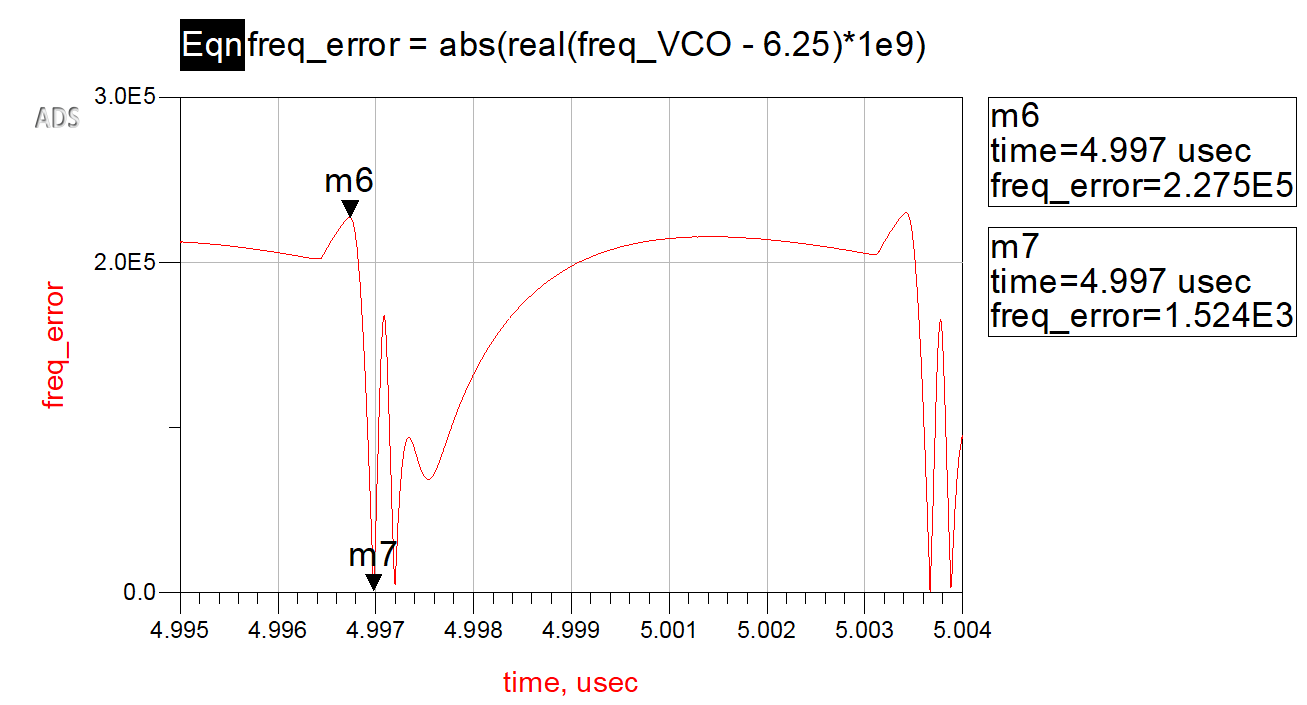
\includegraphics[width=0.5\linewidth]{images/ads_results/real_pll/freq_error_VCO_real.png}%
    \label{fig:freq_error_VCO_real}}
    \hfil
    \subfloat[]{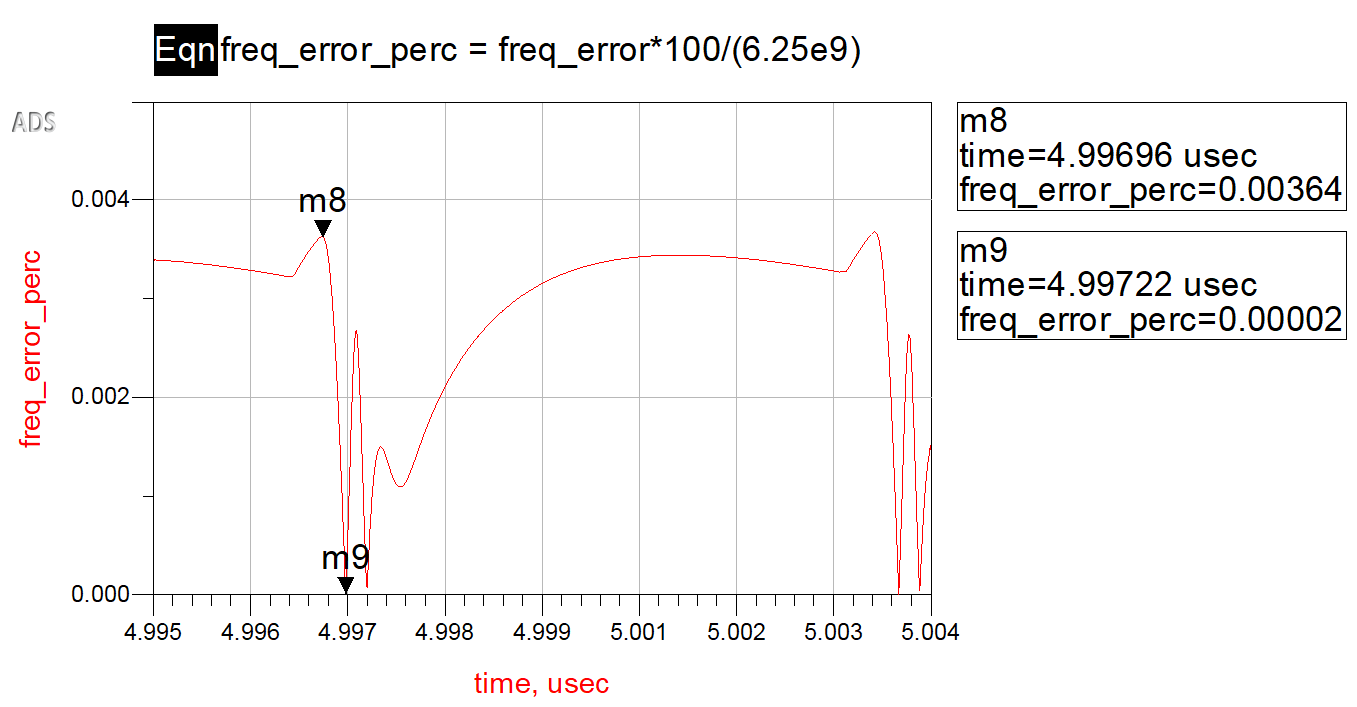
\includegraphics[width=0.5\linewidth]{images/ads_results/real_pll/freq_error_perc_VCO_real.png}%
    \label{fig:freq_error_perc_VCO_real}}
    \hfil
    \caption{Real simulation: (a) Frequency output over time, (b) Frequency over time zoomed, (c) Frequency output error over time, (d) Frequency output error percentage over time.}
    \label{fig:freq_VCO_real_and_zoom}
\end{figure*}

\begin{figure}[!h]
    \centering
    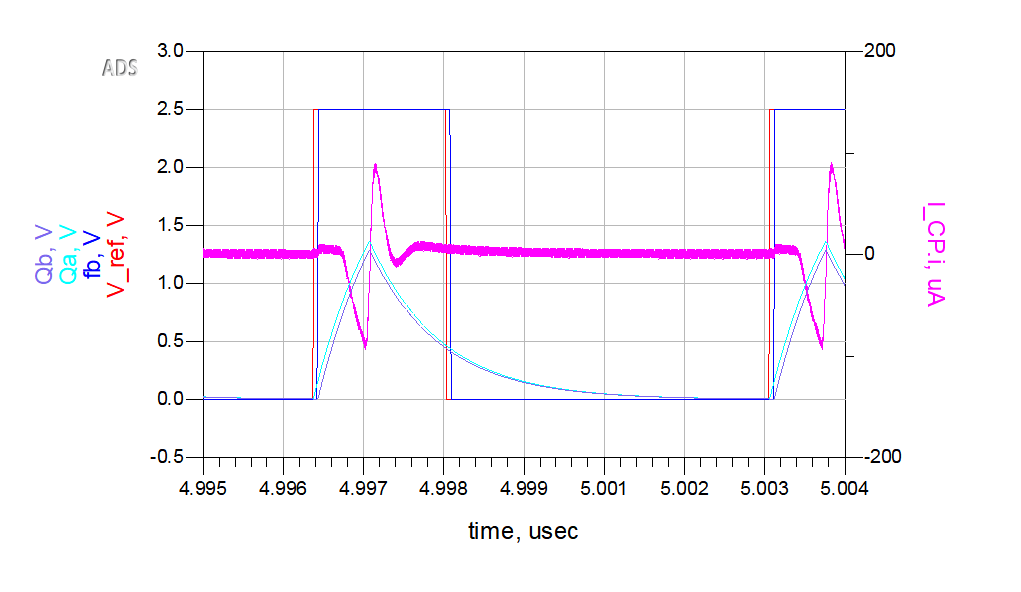
\includegraphics[width=1\linewidth]{images/ads_results/real_pll/Vref_Vfb_real.png}
    \caption{Real simulation: Reference and Feedback voltages over time, compared with Qa, Qb and Icp.}
    \label{fig:Vref_Vfb_real}
\end{figure}

Then, in Fig.~\ref{fig:Vref_Vfb_real}, the inputs of the phase-frequency detector (PFD), its output, and the output current of the charge pump are shown when the system is in steady state. As observed, the difference between \( V_{\text{ref}} \) and \( V_{\text{fb}} \) is mainly attributed to the use of behavioral flip-flops in the phase-frequency detector, as discussed in the section~\ref{sec:block_design}. In any real implementation, there will always be a small difference between the two rising edges due to non-idealities. The observed difference between the rising edges is \(65 \, \text{ps}\), which corresponds to \(8 \times \text{TimeStep}\) in the simulation. Even if the edges were perfectly simultaneous, spurious peaks would still appear, as seen in this case, due to the inherent limitations of the real implementation.

\newpage
\subsection{Frequency Step Response}
\label{sec:freq_step}
\begin{figure*}[!ht]
    \centering
    \subfloat[]{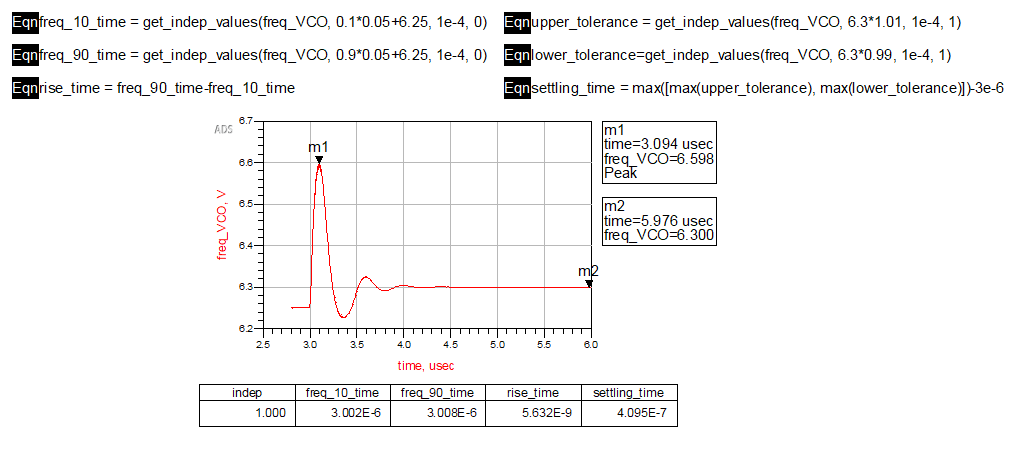
\includegraphics[width=0.5\linewidth]{images/ads_results/freq_step/real_measure.png}%
    \label{fig:freq_step_real_meas}}
    \hfil
    \subfloat[]{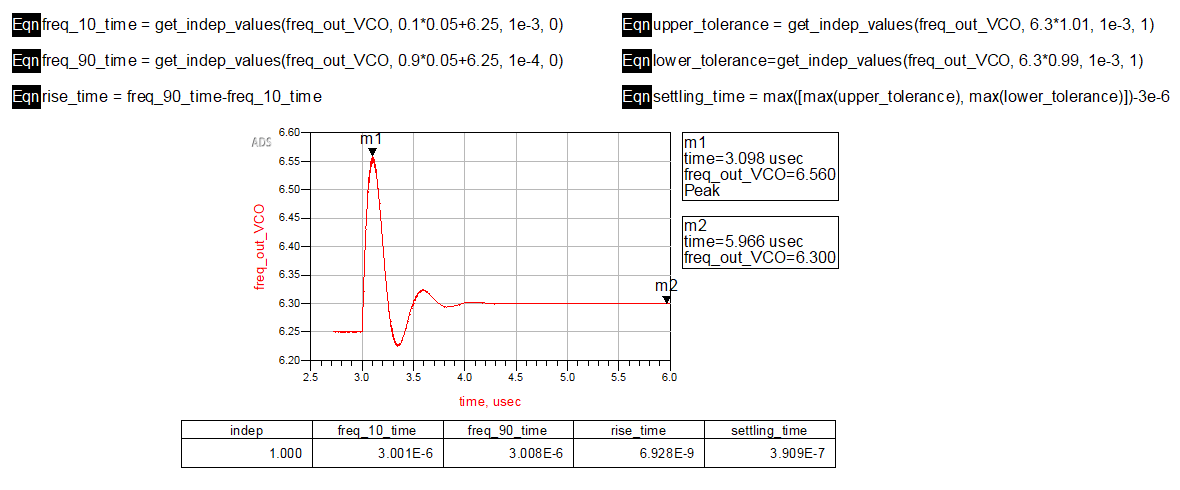
\includegraphics[width=0.5\linewidth]{images/ads_results/freq_step/ideal_measure.png}%
    \label{fig:freq_step_ideal_meas}}
    \hfil
    \caption{Simulation results for an input frequency step on (a) the real and (b) the ideal PLL models. Rise times and 1\% tolerance ($\pm\SI{63}{\mega\hertz}$) settling times are reported.}
    \label{fig:freq_step_results}
\end{figure*}

In this section, the results of the simulations for the PLL’s response to a frequency variation are presented. The simulations begin from steady-state conditions, with the system initially locked at \(6.25 \, \text{GHz}\). At \(t=\SI{3}{\micro\second}\), a frequency step of \(50 \, \text{MHz}\) is applied to \texttt{Vref}, bringing the final frequency to \(6.30 \, \text{GHz}\). 

The simulations are conducted for both the ideal and real-phase locked loop (PLL) systems. The responses are compared to highlight differences in behavior under this dynamic condition.
The used simulation environment for the real and ideal PLL system are shown in figures \ref{fig:freq_step_schem_real} and \ref{fig:freq_step_schem_ideal}.

\begin{figure}[!h]
    \centering
    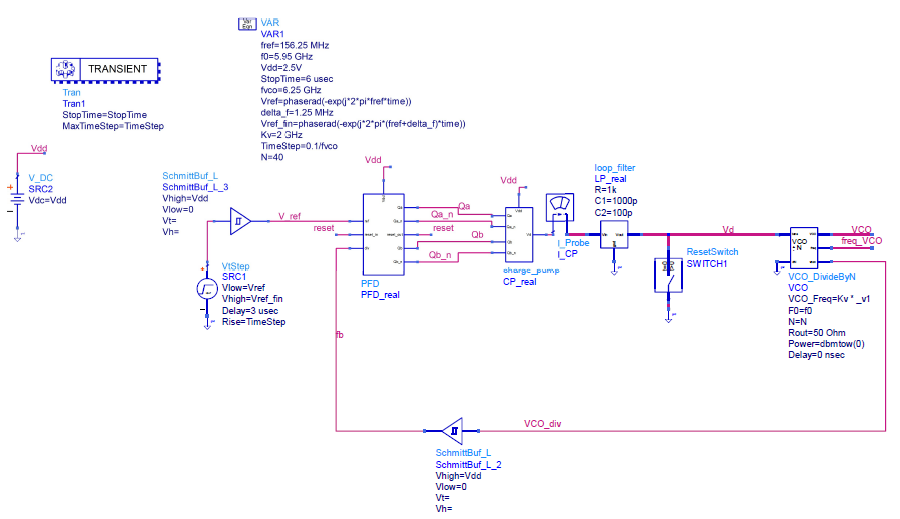
\includegraphics[width=\linewidth]{images/ads_results/freq_step/schematic_real.png}
    \caption{Simulation testbench for the input frequency step on the real PLL model.}
    \label{fig:freq_step_schem_real}
\end{figure}

\begin{figure}[!h]
    \centering
    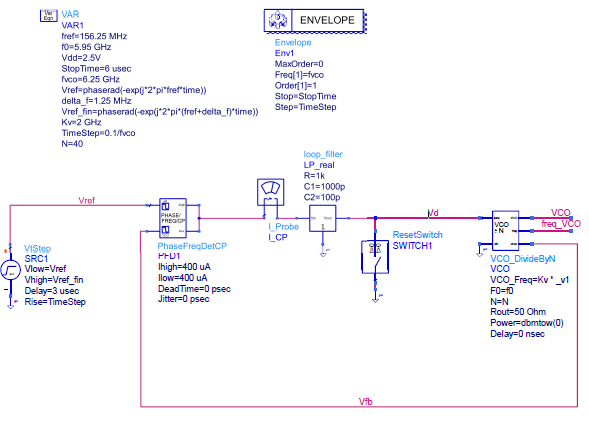
\includegraphics[width=\linewidth]{images/ads_results/freq_step/schematic_ideal.png}
    \caption{Simulation testbench for the input frequency step on the ideal PLL model.}
    \label{fig:freq_step_schem_ideal}
\end{figure}

Again, here as well it was possible to use a faster envelope simulation only for the ideal model, because in the real model the PFD flip-flops are only triggered with a transient simulation, as explained before. The input frequency step is modeled using a \texttt{VtStep} component, stepping from an input signal with phase

\[2\pi f_{ref}\cdot time\]

to a signal with phase

\[2\pi \left(f_{ref}+\Delta f\right)\cdot time\]

where $\Delta f=\SI{1.25}{\mega\hertz}$.

The output results of the simulation are shown in Fig. \ref{fig:freq_step_results}.

As we can see, the rise time in the real model is shorter than the one in the ideal case, whereas the opposite happens for the settling times. This can be easily explained if we observe the time evolution of the charge pump output current (figures \ref{fig:freq_step_real_currents} and \ref{fig:freq_step_ideal_currents}).

\begin{figure}[!h]
    \centering
    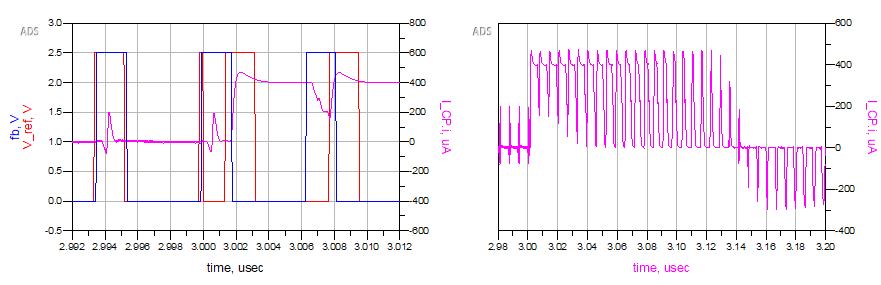
\includegraphics[width=1\linewidth]{images/ads_results/freq_step/real_step.png}
    \caption{Time evolution of the charge pump output current with an input frequency step in the real PLL model.}
    \label{fig:freq_step_real_currents}
\end{figure}

\begin{figure}[!h]
    \centering
    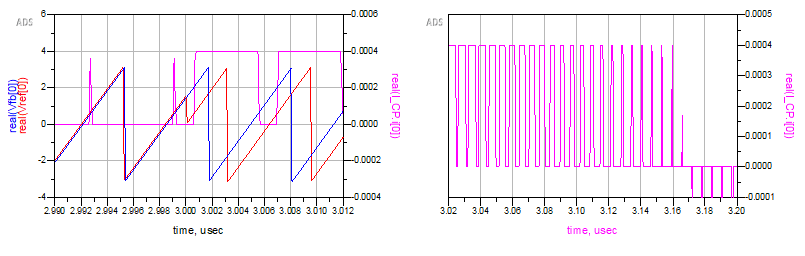
\includegraphics[width=1\linewidth]{images/ads_results/freq_step/ideal_step.png}
    \caption{Time evolution of the charge pump output current with an input frequency step in the ideal PLL model.}
    \label{fig:freq_step_ideal_currents}
\end{figure}

Due to the real response of the designed charge pump, characterized by non-negligible delay times, when a frequency step occurs the output current in the real case rarely manages to drop back to 0 and, therefore, the average value of the charge pump current is higher compared to the ideal case, where the current is characterized by sharp edges. Moreover, current overshoots contribute to increase its average value. As explained in Section\ref{sec:system_level_analysis}, the charge pump current value is equivalent to the proportional gain of the open-loop system, hence the increased responsiveness of the closed-loop system. However, a higher proportional gain also increases the overshoots heights and reduces the stability of the system and for this reason, the settling time in the real case is higher compared to the ideal case.

It is important to observe that residual phase error is almost zero, as shown in Fig. \ref{fig:phase_error_real}

\begin{figure}[!h]
    \centering
    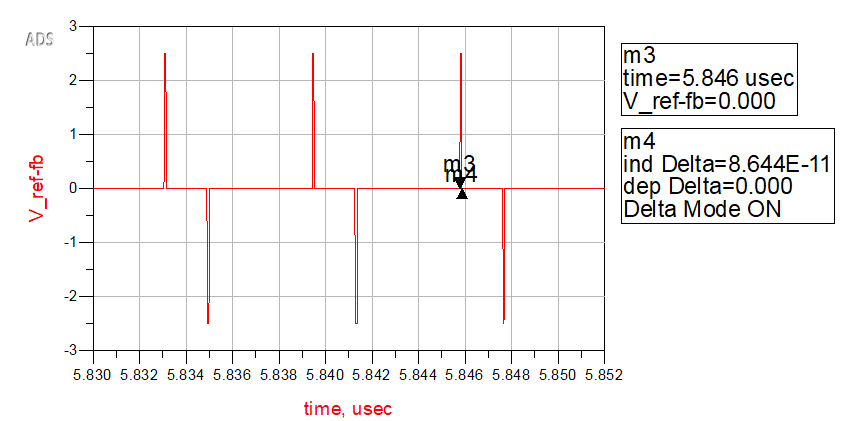
\includegraphics[width=0.5\linewidth]{images/ads_results/freq_step/phase_error_real.png}
    \caption{Residual phase error after the frequency step in the real case.}
    \label{fig:phase_error_real}
\end{figure}

The delay between the reference signal and the feedback signal is of \qty{86.44}{\pico\second}, which is negligible compared to the reference period $\frac{1}{f_{ref}}$. This is possible only thanks to the type of PLL that we implemented (a type-II PLL) and a significant phase error would be present for other types of PLL (type-I) under the same test conditions. This will be studied in Section \ref{sec:comparison}.

\subsection{Phase Step Response}\label{ssec:phase_step}
In this section, the results of the simulations for the PLL’s response to a phase variation of the reference are presented. The simulations begin from steady-state conditions, with the system initially locked at \(6.25 \, \text{GHz}\). At \(t=\SI{3}{\micro\second}\), a phase step of \(\pi \, \text{rad}\) is applied to \texttt{Vref}.

The real and ideal simulation testbenches are the same used for the frequency step test (figures \ref{fig:freq_step_schem_real} and \ref{fig:freq_step_schem_ideal}). However, this time the reference input is stepped from

\[2\pi f_{ref}\cdot time\]

to

\[2\pi f_{ref}\cdot time+\Delta\theta\]

with $\Delta\theta=\pi\ \text{rad}$.

\begin{figure}[!ht]
    \centering
    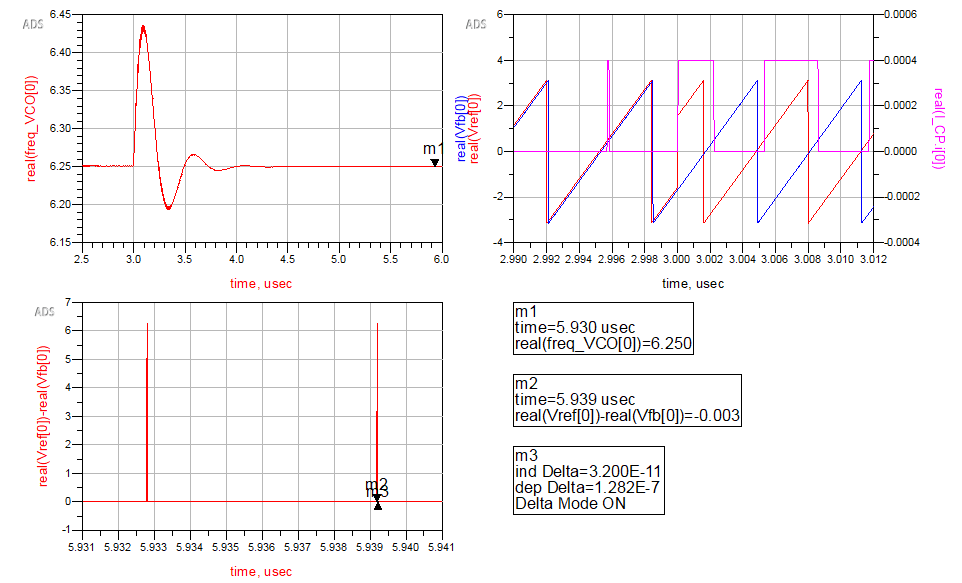
\includegraphics[width=1\linewidth]{images/ads_results/phase_step/phase_step_ideal.png}
    \caption{Simulation results for a phase step of the input in the ideal PLL model.}
    \label{fig:phase_step_ideal_res}
\end{figure}

\begin{figure}[!ht]
    \centering
    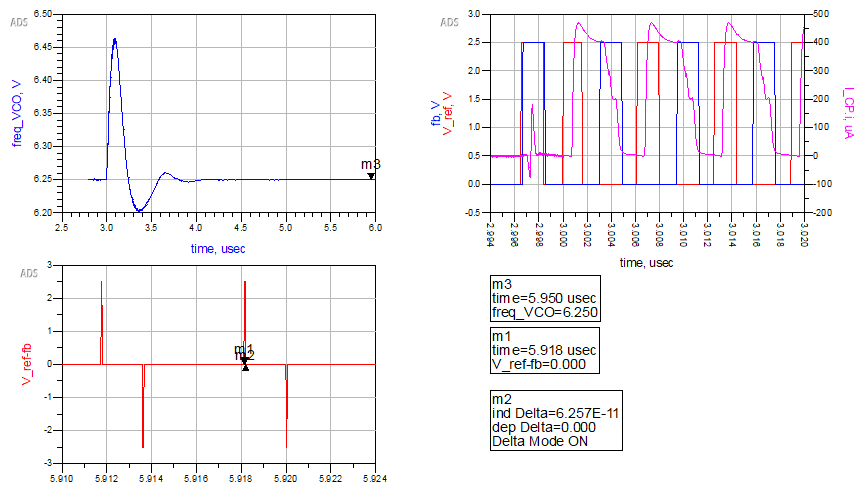
\includegraphics[width=1\linewidth]{images/ads_results/phase_step/phase_step_real.png}
    \caption{Simulation results for a phase step of the input in the real PLL model.}
    \label{fig:phase_step_real_res}
\end{figure}

As we can see from the results shown in figures \ref{fig:phase_step_ideal_res} and \ref{fig:phase_step_real_res}, after an initial oscillation of the VCO frequency, the PLL locks back again to the original frequency of $\SI{6.25}{\giga\hertz}$ with a very small skew ($\SI{62.57}{\pico\second}$ in the real case), which is due to the non-idealities of the PFD and charge pump \cite{razavi_current_mismatch}.

\subsection{Phase Noise}
\label{sec:phase_noise}

This section focuses on determining the phase noise difference between a simple open-loop VCO and the closed-loop PLL solution. For simplicity, the analysis considers the ideal PLL, with all blocks implemented behaviorally. 

The noise source is assumed to originate solely from the voltage-controlled oscillator (VCO). To achieve realistic results, the phase noise of a 65 nm VCO implementation, as presented in \cite{vco}, is used as a case study. Although this work targets a different technology, the purpose is to observe trends rather than provide an exact representation. The open-loop phase noise values for an LC-tank VCO, as reported in the reference, are summarized in Table~\ref{tab:vco_phase_noise}. 

\begin{table}[!ht]
    \renewcommand{\arraystretch}{1.5}
    \centering
    \caption{Open-loop phase noise of the VCO (Ref.~\cite{vco}).}
    \label{tab:vco_phase_noise}
    \begin{tabular}{|c|c|}
        \hline
        \textbf{Frequency Offset [Hz]} & \textbf{Phase Noise [dBc/Hz]} \\ \hline
        \(10^2\)                        & \(-18\)                     \\ \hline
        \(10^3\)                        & \(-41\)                     \\ \hline
        \(10^4\)                        & \(-64\)                     \\ \hline
        \(10^5\)                        & \(-87\)                     \\ \hline
        \(10^6\)                        & \(-110\)                    \\ \hline
        \(10^7\)                        & \(-132\)                    \\ \hline
        \(10^8\)                        & \(-152\)                    \\ \hline
    \end{tabular}
\end{table}

The values in Table~\ref{tab:vco_phase_noise} are interpolated linearly to obtain the phase noise of the VCO at arbitrary frequency offsets.

\begin{figure}[!ht]
    \centering
    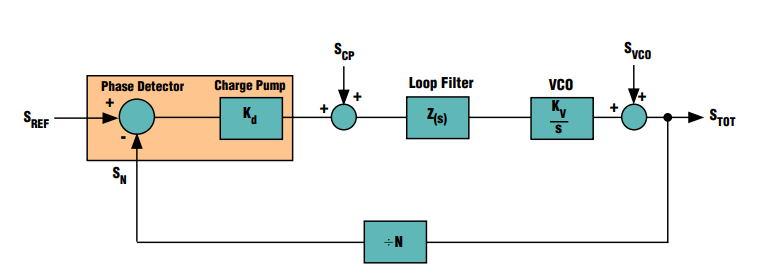
\includegraphics[width=1\linewidth]{images/ads_results/phase_noise/phase_noise_block_schematic.png}
    \caption{Phase-Noise contributors in a PLL circuit.}
    \label{fig:phase_noise_block_schematic}
\end{figure}

Before analyzing the results of introducing phase noise into the PLL chain, we are first interested in deriving the expression for the closed-loop phase noise as it relates to the open-loop phase noise. If, in our case, the reference input does not exhibit phase noise, the PLL aims to minimize the output phase noise to zero, even if the VCO exhibits its own phase noise. In fact, as the VCO phase noise accumulates and becomes appreciable, the loop detects this error and commands the charge pump to briefly turn on and correct it.

To formulate the PLL output noise due to the VCO phase noise, we first derive the transfer function from the VCO phase to the PLL output phase. In Fig.~\ref{fig:phase_noise_block_schematic}, a generic schematic of the contributors to phase noise in a PLL is shown. As mentioned earlier, we focus only on the VCO phase noise (\(S_{\text{VCO}}\)).

The derived transfer function is:

\[
H_n(s) = \frac{\theta_{n,\text{cl}}(s)}{\theta_n(s)} = \frac{N \cdot s}{N \cdot s + K_{\text{VCO}} \cdot Z(s) \cdot \frac{I_{\text{CP}}}{2\pi}},
\]

where, in a similar manner to what was done in Sec.~\ref{sec:system_level_analysis}, we consider the PFD/CP gain \(K_d = \frac{I_{\text{CP}}}{2\pi}\), the loop filter response as \(Z(s)\), \(K_v = K_{\text{VCO}}\) and \(N = 40\).

\begin{figure}[!ht]
    \centering
    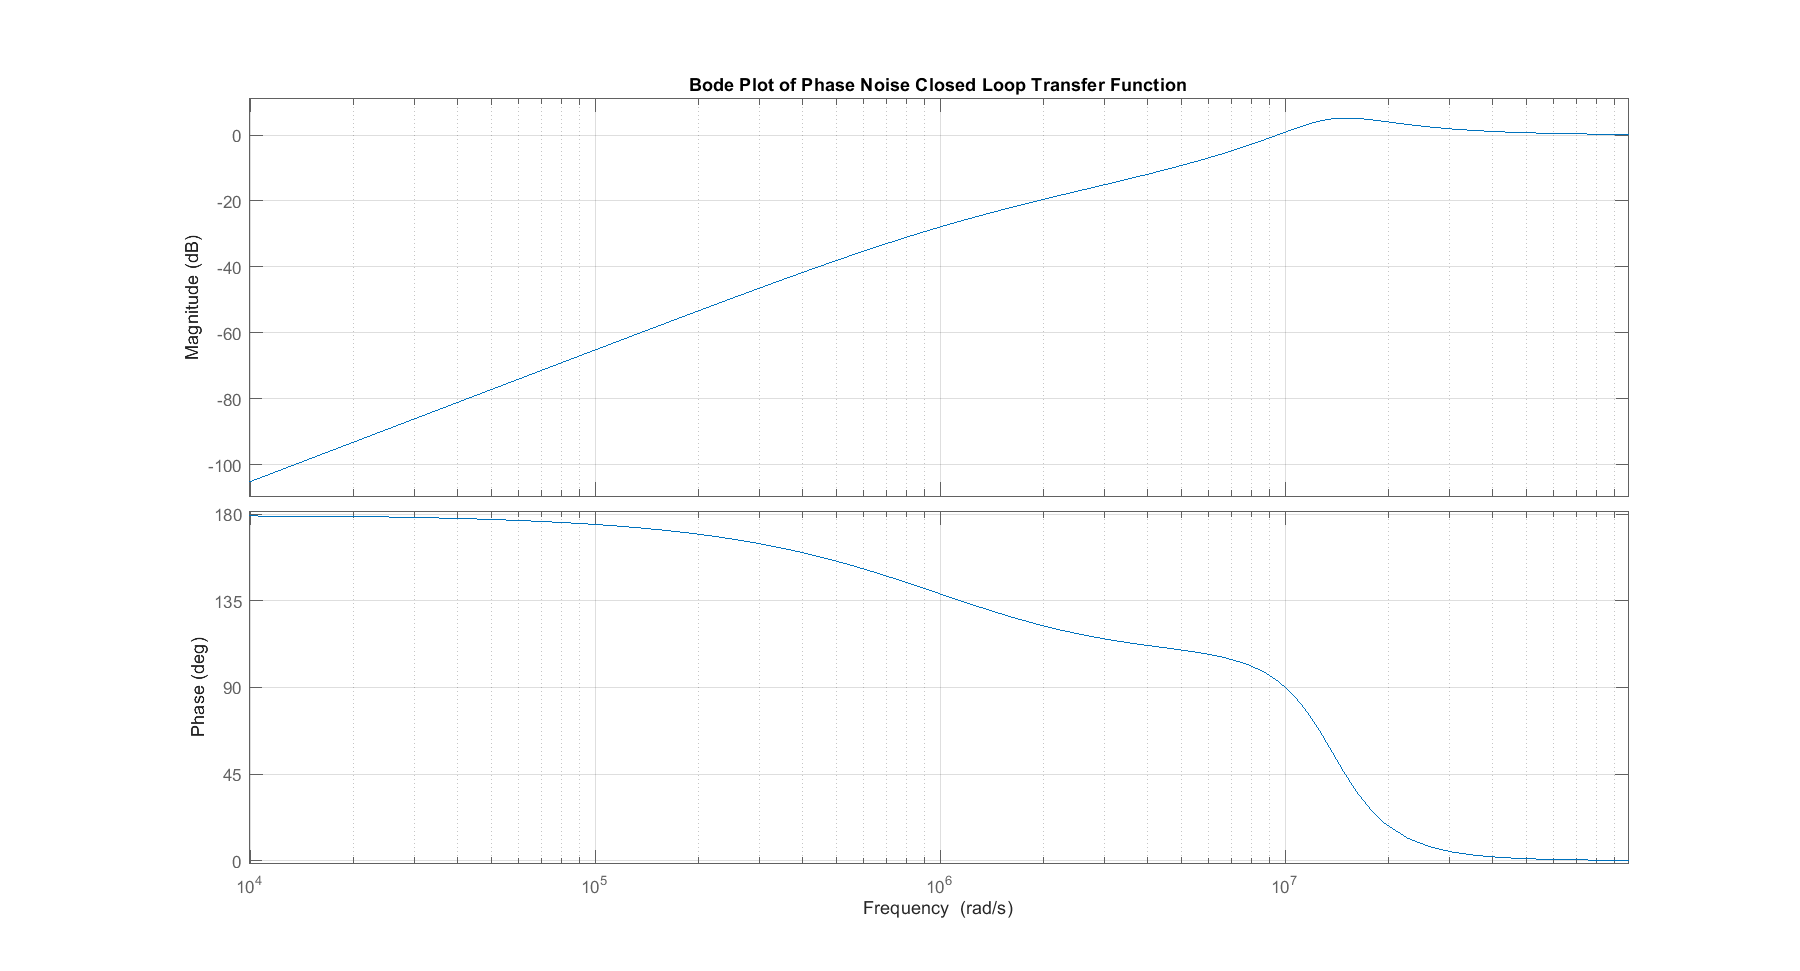
\includegraphics[width=1\linewidth]{images/ads_results/phase_noise/phase_noise_plots.png}
    \caption{Phase noise closed loop over input VCO phase noise bode plots.}
    \label{fig:phase_noise_bode}
\end{figure}

Fig.~\ref{fig:phase_noise_bode} shows the results obtained in MATLAB, demonstrating a classical high-pass response with a corner frequency of approximately \(f_h = 2.5 \, \text{MHz}\).

\begin{figure*}[!ht]
    \centering
    \includegraphics[width=1\linewidth]{images/ads_results/phase_noise/phase_noise.png}
    \caption{ADS schematic used to introduce phase-noise.}
    \label{fig:phase_noise}
\end{figure*}

In order to simulate the VCO phase noise, the circuit shown in Fig.~\ref{fig:phase_noise} is implemented. The lower part of the schematic corresponds to the same PLL charge pump with behavioral components described in Sec.~\ref{sec:block_design}, while the upper part of the schematic introduces phase noise into the chain. This is accomplished through the following components:

\begin{itemize}
    \item A VCO ideal component generates the sinusoidal signal at \(f_{\text{vco}}\) frequency, with a gain \(K_{\text{vco}} = 2 \, \text{GHz/V}\), as described in Sec.~\ref{sec:block_design}. The output is used as an input to a phase modulator.
    \item The phase modulator incorporates a noise source to modulate the phase. The noise source is implemented using a source noise generator, whose values are provided through a \texttt{.mdif} file. This file reproduces the phase noise values represented in Tab.~\ref{tab:vco_phase_noise} via a \(DataAccessComponent\), an ADS custom block used to simulate realistic behavior by interpolating the values provided in the referenced file. Note that the values in the file are in linear scale, as they correspond to phase noise originally represented in dB scale.
    \item To retrieve the open-loop phase noise, a phase demodulator is used after the phase modulator.
    \item To insert the phase noise into the closed loop, a frequency demodulator is employed to obtain the instantaneous frequency. This value is then introduced into the loop using a voltage-controlled generator.
    \item Finally, using the VCO output and another phase demodulator, the closed-loop phase noise is retrieved.
\end{itemize}

This simulation is carried out using an envelope simulation, which reduces CPU simulation time, thanks to the use of behavioral blocks.

The generated phase noise is then integrated into the feedback chain by feeding the noise-modulated VCO output to the rest of the circuit. This ensures that the phase noise propagates through the loop, allowing closed-loop analysis. By modeling the noise behavior in this way, it becomes possible to evaluate the impact of phase noise in both open-loop and closed-loop configurations, as shown in Fig.~\ref{fig:phase_noise}.

\begin{figure*}[!ht]
    \centering
    \includegraphics[width=1\linewidth]{images/ads_results/phase_noise/phase_noise_results.png}
    \caption{Phase noise results.}
    \label{fig:phase_noise_results}
\end{figure*}

In Fig.~\ref{fig:phase_noise_results}, the results of the open-loop and closed-loop phase noise simulations are shown. These results include both the FFT of the VCO outputs and the phase noise observed after the phase demodulators.

As can be seen from Fig.~\ref{fig:phase_noise_results}, the open-loop phase noise (PN\textsubscript{OL}) at \(1 \, \text{MHz}\) is: 
\[
PN_{\text{OL}} (@ 1 \, \text{MHz}) =  -45.93 \, \text{dBc/Hz}, 
\]
while the closed-loop phase noise (PN\textsubscript{CL}) at \(1 \, \text{MHz}\) is: 
\[
PN_{\text{CL}} (@ 1 \, \text{MHz}) =  -82.496 \, \text{dBc/Hz}. 
\]
Additionally, a peak at \(1.977 \, \text{MHz}\) is observed with a value of \(-43.179 \, \text{dBc/Hz}\). These results confirm the findings of the theoretical calculation for the phase noise transfer function, which predicts a high-pass response with an overshoot near \(2.5 \, \text{MHz}\). In the simulation, a peak is observed at \(2 \, \text{MHz}\) in the closed-loop phase noise, while the open-loop phase noise continues to diminish, as described in \cite{vco}.

It is important to note that the loop filter design was not optimized with specific constraints imposed by phase noise requirements. Therefore, it is possible to fine-tune the loop filter parameters to reduce the phase noise further, if necessary.

\newpage
\section{Comparison with a Type-I PD-PLL}\label{sec:comparison}
A type-I PLL is a simpler version of phase-locked loop, where the number of integrators reduces to 1, i.e. only the VCO with its transfer function equal to $\frac{K_{VCO}}{s}$. The model of the PLL is equivalent to the one shown in Fig. \ref{fig:type_one_pll_blocks}. The frequency divisor in the feedback loop can be still implemented, if we are interested in a frequency multiplication.

\begin{figure}[!h]
    \centering
    \includegraphics[width=1\linewidth]{images/type_one_pll/block_schematic.png}
    \caption{Block schematic of a type-I PLL}
    \label{fig:type_one_pll_blocks}
\end{figure}

This type of PLL does not have a phase-frequency detector, because the charge pump and the integrator introduced by the previous loop filter are not present. It only has a simple phase-detector, where the output $V_e$ is proportional to the error between the phase of the reference and the phase of the frequency divided VCO output. An ideal phase detector can be modeled as in Fig. \ref{fig:pd_schematic}.

\begin{figure}[!h]
    \centering
    \includegraphics[width=1\linewidth]{images/type_one_pll/pd_schematic.png}
    \caption{Block view of a phase detector and ideal output characteristic.}
    \label{fig:pd_schematic}
\end{figure}

One real implementation of this block is using a reset dominant SR flip-flop, where the reference signal is connected to the set input and the feedback to the reset. The square waveform at the output of the flip-flop can then be smoothed out using a first order RC low-pass filter and the average value of $\frac{V_{DD}}{2}$ can be removed using a subtractor. The resulting $V_e$ output characteristic of this block is shown in Fig. \ref{fig:output_srff}.

\begin{figure}[!h]
    \centering
    \includegraphics[width=1\linewidth]{images/type_one_pll/srff_output.png}
    \caption{Output characteristic of a PD implemented using a SR flip-flop}
    \label{fig:output_srff}
\end{figure}

The output of the PD can be additionally filtered using a first order low pass loop filter with one real negative pole. This is shown in Fig. \ref{fig:type_one_pll_blocks}, where the loop filter is represented by the $R_1-C_1$ group. Notice that, if the loop filter had a real pole in $s=0$ (accurately compensated by a real zero to avoid instability), the number of integrators in the loop would be two and the system would become again a type-II PLL. Therefore, in this case, the loop filter transfer function is given by:

\begin{equation}\label{eq:loop_filter_tf_type_one}
    F(s)=\frac{1}{1+sR_1C_1}
\end{equation}

We can now obtain the closed-loop transfer function of the phase-domain model shown in Fig. \ref{fig:phase_dom_model_type_one}.

\begin{figure}
    \centering
    \includegraphics[width=1\linewidth]{images/type_one_pll/phase_domain_model.png}
    \caption{Phase-domain model of a type-I PLL.}
    \label{fig:phase_dom_model_type_one}
\end{figure}

Here, $K_{VCO}$ is again equal to $\qty[per-mode = symbol]{2}{\giga\hertz\per\volt}=\qty[per-mode=symbol]{12.57}{\kilo\radian\per\volt}$, whereas the constant gain of the phase detector $K_{PD}$ can be calculated from the output characteristic of Fig. \ref{fig:output_srff} and it is equal to $\frac{V_{DD}}{2\pi}\ \unit[per-mode=symbol]{\volt\per\radian}$. The output frequency is again divided by $N=40$.
The open-loop gain is equal to:

\begin{equation}\label{eq:open_loop_gain}
    G(s)=\frac{K_{PD}K_{VCO}F(s)}{s}
\end{equation}

As obtained in \cite{razavitypeone}, the closed-loop transfer function is then equal to:

\begin{equation}\label{eq:type_one_tf}
    H(s)=\frac{\theta_{out}}{\theta_{in}}(s)=\frac{\frac{K_{PD}K_{VCO}}{N}}{R_1C_1s^2+s+\frac{K_{PD}K_{VCO}}{N}}
\end{equation}

That can be seen as

\begin{equation}\label{eq:type_one_tf_bis}
    H(s)=\frac{\omega_n^2}{s^2+2\zeta\omega_ns+w_n^2}
\end{equation}

where

\begin{equation}\label{eq:damping_factor}
    \zeta=\frac{1}{2}\sqrt{\frac{N\omega_{LPF}}{K_{PD}K_{VCO}}}
\end{equation}

\begin{equation}\label{eq:resonance_freq}
    \omega_n=\sqrt{\frac{K_{PD}K_{VCO}\omega_{LPF}}{N}}
\end{equation}

and $\omega_{LPF}=1/R_1C_1$. The damping factor is typically chosen to be $\sqrt{2}/2$ or larger so as to provide a critically-damped or overdamped response. Using the final value theorem, we can also define a DC loop gain:

\begin{equation}\label{eq:dc_gain}
    K_{DC}=\underset{s\to 0}{\lim}\left(\frac{sG(s)}{N}\right)=\frac{K_{PD}K_{VCO}F(0)}{N}
\end{equation}

Notice that the closed-loop transfer function for the phase is the same for the frequencies:

\begin{equation}\label{eq:same_tf}
    \frac{\Omega_{out}}{\Omega_{in}}(s)=\frac{\theta_{out}s}{\theta_{out}s}(s)=H(s)
\end{equation}

This means that when an input frequency step occurs, after some transient the output frequency will be equal to the new input frequency).

However, the problem with this type of PLL is that there will always be some residual phase error when the reference input undergoes a frequency step. This can be seen by analyzing the error transfer function:

\begin{equation}\label{eq:error_tf}
    E(s)=\frac{\theta_{in}-\theta_{out}/N}{\theta_{in}}(s)=\frac{s}{s+\frac{K_{PD}K_{VCO}F(s)}{N}}
\end{equation}

Notice that here the type of the PLL is not specified and $F(s)$ is kept implicit.
When we apply a phase step $\theta_{in}=\Delta\theta u(t)$, the steady-state error will be:

\begin{equation}\label{eq:err_phase_step}
    \theta_{err}=\underset{s\to 0}{\lim}\left(\frac{\Delta\theta}{s}\right)\left(sE(s)\right)=0
\end{equation}

independently from the type of PLL chosen.
On the other hand, when we apply a frequency step $f_{in}=\Delta f u(t)$, which corresponds to an input phase ramp:

\begin{equation}\label{eq:err_freq_step}
    \theta_{err}=\underset{s\to 0}{\lim}\left(\frac{\Delta f}{s^2}\right)\left(sE(s)\right)=\frac{\Delta f}{K_{DC}}
\end{equation}

and now we can see that if the loop lacks of an additional integrator, which allows to obtain an infinite DC gain, there will always be a phase error upon an input frequency step, even though the type-I PLL still manages to lock the output frequency to the input frequency, as shown with equation \ref{eq:same_tf}.

\medskip
Now, we can reproduce this result by modeling a type-I PLL using ADS. The schematic of the model is shown in Fig. \ref{fig:type_one_ads_model}.

\begin{figure*}[!ht]
    \centering
    \includegraphics[width=1\linewidth]{images/type_one_pll/ADS_schematic.png}
    \caption{Schematic view of a type-I PLL model in ADS.}
    \label{fig:type_one_ads_model}
\end{figure*}

The SR flip-flop was set to produce a digital output with logic level at \qty{0}{\volt} and \qty{2.5}{\volt} ($V_{DD}$), with rise and fall times such that its equivalent bandwidth - approximately equal to $\frac{0.35}{t_{rise}}$ - is larger than the reference frequency of \qty{156.25}{\mega\hertz}. The RC group outside the SR flip-flop is used to smooth out the higher frequency components introduced by the flip-flop: its bandwidth was chosen to be much smaller than $f_{ref}$, in particular it was set to \qty{1.56}{\mega\hertz}, with $R=\qty{1}{\kilo\ohm}$ and $C=\qty{102}{\pico\farad}$. This filtered voltage, \texttt{Vpd\_filterd}, is then summed to a constant value of $-\frac{V_{DD}}{2}$, in order to remove its average value, as explained before.

The loop filter was designed so that the system is critically-damped

\begin{equation}
    \zeta=\frac{\sqrt{2}}{2} \Longrightarrow \omega_{LPF}=2\frac{K_{PD}K_{VCO}}{N}=\qty[per-mode=symbol]{250e6}{\radian\per\second}
\end{equation}

The following values for the RC group were chosen:

\[R_1=\qty{1}{\kilo\ohm},\ C_1=\qty{4}{\pico\farad}\]

\subsection{Phase Step}

Using similar testbenches as the ones used for our type-II PLL (see Fig. \ref{fig:freq_step_schem_real}), a phase step and a frequency step were applied to the type-I PLL.

\begin{figure}[!h]
    \centering
    \includegraphics[width=0.75\linewidth]{images/type_one_pll/phase_step_type_one.png}
    \caption{Output frequency of a type-I PLL with an input phase step.}
    \label{fig:type_one_phase_step}
\end{figure}

The system, after some transient, is locked at the central resonance frequency of the VCO $f_0=\qty{5.95}{\giga\hertz}$, using an input reference frequency $f_{ref}=\frac{f_0}{N}=\qty{148.75}{\mega\hertz}$. At $t=\qty{10}{\micro\second}$ a phase step of $\pi\ \unit{\radian}$ is applied. In Fig. \ref{fig:type_one_phase_step} we can see how the output frequency changes when the step is applied, but, after some time, the output frequency goes back to $f_0$.

In Fig. \ref{fig:type_one_phase_step_error}, we can see that the average value of the voltage $V_e$, proportional to the phase error, eventually goes back to 0, as we proved before in our model. The same happened for the type-II PLL, as discussed in Section \ref{ssec:phase_step}.

\begin{figure}[!h]
    \centering
    \includegraphics[width=1\linewidth]{images/type_one_pll/phase_step_error.png}
    \caption{Averaged output voltage of the phase detector $V_e$ in a type-I PLL with an input phase step.}
    \label{fig:type_one_phase_step_error}
\end{figure}

\subsection{Frequency Step}
In a similar manner to the previous section, a frequency step from $f_0=\qty{5.95}{\giga\hertz}$ to $f_1=\qty{6.25}{\giga\hertz}$ was applied.

\begin{figure}[!h]
    \centering
    \includegraphics[width=1\linewidth]{images/type_one_pll/freq_step_type_one.png}
    \caption{Output frequency of a type-I PLL with an input frequency step.}
    \label{fig:type_one_freq_step}
\end{figure}

\begin{figure}[!h]
    \centering
    \includegraphics[width=1\linewidth]{images/type_one_pll/freq_step_error.png}
    \caption{Averaged output voltage of the phase detector $V_e$ in a type-I PLL with an input phase step.}
    \label{fig:type_one_freq_step_error}
\end{figure}

As we can see from figures \ref{fig:type_one_freq_step} and \ref{fig:type_one_freq_step_error}, after some transient the output frequency is locked to the new set-point of \qty{6.25}{\giga\hertz}, however, the final phase error voltage $V_e$ is not zero. This can be compared to what happened with the type-II PLL, where the final error was almost zero (see \ref{fig:phase_error_real}). This is one of the main reasons why type-II PLLs are usually preferred over type-I PLLs.
Given the input-output characteristic of the phase detector, as described before, we can calculate the actual difference between the reference and feedback phases:

\[V_e=K_{PD}\left(\theta_{ref}-\theta_{fb}\right) \]

\[\theta_{ref}-\theta_{fb}=\frac{V_e}{K_{PD}}=\frac{\qty{0.15}{\volt}}{\frac{\qty{2.5}{\volt}}{2\pi\ \unit{\radian}}}=\frac{3}{25}\pi\ \unit{\radian}\]

which, at the reference frequency $f_{ref}=\qty{156.25}{\mega\hertz}$, corresponds to a time delay of:

\[\Delta t_{delay}=\frac{\theta_{ref}-\theta_{fb}}{2\pi f_{ref}}=\qty{384}{\pico\second}\]

This value is almost 5 times bigger than the one obtained with the type-II PLL (\qty{86.44}{\pico\second}).

\section{Future Improvements}
\label{sec:future_improvements}

At this point, it is interesting to evaluate the potential future improvements for the 6.25 GHz PLL designed for the SpaceFibre standard. Several enhancements can be explored to increase the performance, robustness, and compliance with the standard. These improvements can be categorized at the system level, circuit level, and simulation level.

First, at the system level, it would be crucial to focus more on radiation-hardened (rad-hard) improvements to ensure compliance with the SpaceFibre standard, especially for applications in space. One significant future improvement could involve adopting a triple-modular redundancy (TMR) module for the Phase Frequency Detector (PFD). The block schematic for this TMR configuration is shown in Fig.~\ref{fig:tmr}. This approach improves the reliability of the PLL by providing fault detection and correction, allowing the system to continue operating in the presence of faults or radiation-induced failures. TMR provides increased fault tolerance and enhances the PLL’s robustness in environments where radiation or other disruptions could affect the performance.

\begin{figure}
    \centering
    \includegraphics[width=1\linewidth]{images/future_improvements/tmr.png}
    \caption{TMR implementation.}
    \label{fig:tmr}
\end{figure}

At the circuit level, it would be valuable to investigate alternative implementations of the charge pump. For example, as discussed in \cite{original}, using a differential input stage in the charge pump could be beneficial. A differential input stage would allow for reduced electromagnetic interference (EMI), which is crucial for high-frequency designs. Specifically, an Enhanced Charge Pump (CP) Gate Switching architecture with differential inputs has been found to reduce EMI and improve overall efficiency. This architecture can result in more stable and less noisy performance, which would be highly beneficial for PLL operation in demanding environments.

From a simulation perspective, a significant future improvement could be to introduce Single Event Effects (SEE) into the charge pump and observe their impact on the PLL's performance. By simulating the effects of SEEs, we can analyze how they influence the PLL's figure of merit, such as stability and accuracy. This would help assess the robustness of the PLL design and identify potential weaknesses that need to be addressed in future iterations, especially in space or other radiation-prone environments.

Another potential improvement could involve implementing a real Voltage-Controlled Oscillator (VCO) and frequency divider using SG25H4 technology. By replacing the modeled VCO and divider with physical components, the design could be tested in real-world conditions, providing more accurate insights into the system's behavior. This would allow the simulations to be validated against actual performance data, and any discrepancies could be addressed by adjusting the design accordingly.

Additionally, phase noise reduction could be a crucial focus for improving the PLL. It could be worthwhile to tune the loop filter in such a way that phase noise is minimized while maintaining other system constraints. As described in Section~\ref{sec:phase_noise}, phase noise is a critical factor for PLL performance, and optimizing the loop filter parameters could lead to better noise rejection and more stable operation, especially in precision applications where low phase noise is required.

Finally, the ultimate step in improving the PLL design would involve layout implementation followed by post-synthesis simulation. Tools such as Cadence Virtuoso could be used to create the physical layout and perform post-synthesis simulations to verify that the PLL functions as expected. This step would allow for the identification and mitigation of parasitic effects introduced during layout, ensuring that the final physical design performs optimally and meets all specified requirements.

\section{Conclusions}
\label{sec:conslusions}
This work presented the design and analysis of a Type-II charge pump PLL operating at \(6.25 \, \text{GHz}\), compatible with the SpaceFibre standard, using the Advanced Design System (ADS) simulation environment. 

The study began with a system-level analysis and design to gain an understanding of the closed-loop response and to appropriately dimension the various PLL components. This included setting target specifications for phase margin, loop bandwidth, and stability criteria, ensuring an efficient and robust design for the case study.

The focus then shifted to the detailed design of key components: the phase-frequency detector (PFD), the charge pump (CP) in the SG25H4 technology, and the loop filter. These components were designed to achieve acceptable phase margins and bandwidth while adhering to the required technological constraints. Each block was implemented and tested individually, showing promising results that validated the designs.

To compare and validate the developed PLL design, an ideal charge pump PLL was also simulated using behavioral ADS blocks. Both the ideal and transistor-level implementations were subjected to frequency and phase step inputs, demonstrating successful locking in both cases with satisfactory dynamic responses.

Furthermore, the effects of VCO phase noise were analyzed by introducing phase noise into the loop and simulating the closed-loop system. The results confirmed the classical high-pass characteristic of phase noise in a Type-II PLL, aligning with theoretical expectations. 

Additionally, the work contrasted the Type-II charge pump PLL with a classical Type-I PLL, focusing on their behavior under frequency and phase step inputs. As expected, while a Type-I PLL can lock to the frequency, it fails to achieve phase locking, resulting in a steady-state phase error. In contrast, the Type-II PLL demonstrated the ability to lock both frequency and phase after a frequency step, showcasing its superior accuracy and completeness as a system.

In summary, this work provides a thorough exploration of the design, implementation, and analysis of a Type-II charge pump PLL, highlighting its advantages over Type-I implementations and its capability to meet the stringent requirements of the SpaceFibre standard.

\printbibliography

\end{document}


